\documentclass[12pt]{book}
\usepackage{fullpage,epic,eepic,epsfig,makeidx,color,moreverb,version,boxedminipage,graphicx}

\includeversion{tobedone}

%\usepackage{lucida}

%\usepackage{t1enc}

\newcommand{\gpl}{Gnu Public License}
\newcommand{\pip}{PiP}
\newcommand{\lpsolve}{LP-Solve}


\newcommand{\sitemmalfa}{\texttt{www.irisa.fr/api/...}}
\newcommand{\alfa}{{\sc Alpha}}
\newcommand{\Alpha}{{\sc Alpha}}
\newcommand{\alfhard}{{\sc AlpHard}}
\newcommand{\AlpHard}{{\sc AlpHard}}
\newcommand{\AlphaZ}{{{\Alpha}0}}
\newcommand{\mma}{{\sc Mathematica}}
\newcommand{\mmalfa}{{\sc MmAlpha}}
\newcommand{\mmalpha}{{\sc MmAlpha}}
\newcommand{\myscale}{1.4}
\newcommand{\Z}{\bf Z}
\newcommand{{\alphaz}}{{\alfa}0}
\newcommand{{\alphard}}{{\alfhard}}
\newcommand{\api}{{\sc api}}
\newcommand{\irisa}{ Irisa}
\newcommand{\vlsi}{{\sc vlsi}}
\newcommand{\vhdl}{{\sc vhdl}}
\newcommand{\Opt}[1]{{\rm\sl [} #1 {\rm\sl ]}}
\newcommand{\Group}[1]{{\rm\sl (} #1 {\rm\sl )}}
\newcommand{\Alt}{$\mid$}
\newcommand{\Program}{{\sl Program\ }}
\newcommand{\PDecl}{{\sl PDecl\ }}
\newcommand{\PointwiseDecl}{{\sl PointwiseDecl\ }}
\newcommand{\SystemDecl}{{\sl SystemDecl\ }}
\newcommand{\Name}{{\sl Name\ }}
\newcommand{\ScalarInDeclList}{{\sl ScalarInDeclList\ }}
\newcommand{\ScalarOutDecl}{{\sl ScalarOutDecl\ }}
\newcommand{\ScalarLocDeclList}{{\sl ScalarLocDeclList\ }}
\newcommand{\ScalarVarDecl}{{\sl ScalarVarDecl\ }}
\newcommand{\ScalarDeclList}{{\sl ScalarDeclList\ }}
\newcommand{\InputDeclList}{{\sl InputDeclList\ }}
\newcommand{\OutputDeclList}{{\sl OutputDeclList\ }}
\newcommand{\LocalDeclList}{{\sl LocalDeclList\ }}
\newcommand{\VarDeclList}{{\sl VarDeclList\ }}
\newcommand{\EquationBlock}{{\sl Equationblock\ }}
\newcommand{\ParamDecl}{{\sl ParamDecl\ }}
\newcommand{\VarDeclaration}{{\sl VarDeclaration\ }}
\newcommand{\Domain}{{\sl Domain\ }}
\newcommand{\IdentifierList}{{\sl IdentifierList\ }}
\newcommand{\Identifier}{{\sl Identifier\ }}
\newcommand{\ScalarType}{{\sl ScalarType\ }}
\newcommand{\IndexList}{{\sl IndexList\ }}
\newcommand{\ConstraintList}{{\sl ConstraintList\ }}
\newcommand{\AffineFunction}{{\sl AffineFunction\ }}
\newcommand{\Constraint}{{\sl Constraint\ }}
\newcommand{\IncreasingSeq}{{\sl IncreasingSeq\ }}
\newcommand{\DecreasingSeq}{{\sl DecreasingSeq\ }}
\newcommand{\EqualitySeq}{{\sl EqualitySeq\ }}
\newcommand{\IndexExpList}{{\sl IndexExpList\ }}
\newcommand{\EquationList}{{\sl EquationList\ }}
\newcommand{\Equation}{{\sl Equation\ }}
\newcommand{\ParamAssignation}{{\sl ParamAssignation\ }}
\newcommand{\InputList}{{\sl InputList\ }}
\newcommand{\ExtParamAssgn}{{\sl ExtParamAssgn\ }}
\newcommand{\ExtensionDomain}{{\sl ExtensionDomain\ }}
\newcommand{\ExpressionList}{{\sl ExpressionList\ }}
\newcommand{\Expression}{{\sl Expression\ }}
\newcommand{\Constant}{{\sl Constant\ }}
\newcommand{\IntegerConstant}{{\sl IntegerConstant\ }}
\newcommand{\RealConstant}{{\sl RealConstant\ }}
\newcommand{\BooleanConstant}{{\sl BooleanConstant\ }}
\newcommand{\BinaryOp}{{\sl BinaryOp\ }}
\newcommand{\CommutativeOp}{{\sl CommutativeOp\ }}
\newcommand{\RelativeOp}{{\sl RelativeOp\ }}
\newcommand{\UnaryOp}{{\sl UnaryOp\ }}
\newcommand{\IndexExpression}{{\sl IndexExpression\ }}
\newcommand{\IndexTerm}{{\sl IndexTerm\ }}
\newcommand{\Number}{{\sl Number\ }}
\newcommand{\Digit}{{\sl Digit\ }}
\newcommand{\Letter}{{\sl Letter\ }}

%\newcommand{\}{{\sl \ }}


\newcommand {\setn}   {\hbox{\it I\hskip -2pt N}}     % ensemble N
\newcommand {\setz}   {\hbox{\it Z\hskip -4pt Z}}     %ensemble Z
\newcommand {\setq}   {\hbox{\it Q\hskip -6pt {\it l}\hskip 4pt}}     % ensemble Q


\newcounter{Nex}

\newenvironment{ex}
{\vspace{0.5cm} \refstepcounter{Nex} {\bf Example ${\theNex}$:}
\begin{quotation}}
{\end{quotation}}



\newtheorem{definition}{Definition}[section]





\makeindex
\begin{document}
\title{First Steps in \alfa{}\thanks{Version of \today{}}}

\author{The Alpha team\footnote{Contact: \texttt{alpha@irisa.fr}. See also
\texttt{http://www.irisa.fr/api/ALPHA/welcome.html.}}}

\date{\today}
\maketitle
\tableofcontents
\listoffigures




% abstract = resume the paper
% introduction
% 


% Paper introduction:
% Problem to solve, what exists (related work) and how do we compare to other
% Contributions (3): 3 tensed sentences
% Benchmarks => evaluation metrics, prove introduction statements by evaluation
\subsection*{Abstract}
Dynamic programming is a common pattern of Computer Science to solve problem that follow the Bellman's principle: optimal solutions depends on optimal sub-problem solutions. Solving a dynamic programming problem decomposes in two phases: filling one or more matrices with sub-problems intermediate results and decomposing how the final result was constructed (backtracking). Yet matrices computation formulae and recurrences might be difficult to express, indexing element is often error prone and writing an efficient parallel implementation can take a significant amount of time. In this project, we present \textit{DynaProg}, a language embedded in Scala (DSL) to address dynamic programming problems on heterogeneous platforms. DynaProg allows the programmer to write concise programs based on a pair of parsing grammar and algebra; these program can then be executed either on CPU or on GPU.

We evaluate the performance of our implementation against existing work and own ad-hoc implementations for both the CPU and GPU versions of DynaProg.

Experimental results show an average speedup of {\color{red} XXX} for large problems when they are run on the GPU (compared to CPU). Compared to ad-hoc GPU implementations, the generated parsers have an average slowdown of {\color{red} XXX}.

The CPU implementation has a slowdown of {\color{red} XXX} for {\color{red} PROBLEM} against {\color{red} REF,GAPC?}.
The GPU implementation has a slowdown of {\color{red} XXX} for {\color{red} PROBLEM} against {\color{red} REF,CudAlign, RNAFold}.
 
\vfill
This project has been achieved in collaboration with Manohar Jonnalagedda. I also would like to thank the LAMP team, including Eugene Burmako, Sandro Stucki, Vojin Jovanovic and Tiark Rompf who provided insightful advices and suggestions. I hope you will enjoy your reading. \vspace{.3cm}\\
\textit{Thierry Coppey}

% ------------------------------------------------------------------------------------------------
\newpage
\setcounter{tocdepth}{2} \tableofcontents
\newpage
\section{Introduction}
Dynamic programming (DP) is a technique used to solve combinatorial optimization problems that verify the Bellman's principle: optimal solutions depends on optimal solutions of sub-problem. Dynamic programming often allows to find solutions in an exponential search space (number of solutions) in polynomial running time. The user is usually interested in one optimal solution of the problem, but he might also desire to have \textit{all} optimal solutions (co-optimal), a fixed number of near-optimal solutions, or some synthetic properties of the search space such as its size or the sum of all scores.

Dynamic programming problems arise in several areas of applied Computer Science such as biosequence analysis, natural language processing and operational research. Unfortunately, they appear in multiple variations, and often with a considerable degree of sophistication such that there is a mismatch between textbook solutions and the real-world implementation. Additionally, implementation debugging is tedious and require a lot of time, and little changes in the formulae might imply large rewrites of the matrices and recurrences. \cite{gapc_yield}

For efficiency reasons, the process of dynamic programming computation is split in two: first intermediate scores are memoized in a matrix (tabulation), and reused to construct scores for larger problems; then a backtrack stage retrieve the solution associated with the optimal score for the problem. This solution describes how to obtain the optimal score and is called trace or backtrack trace, and heavily depends on the matrix design. The obtained information then needs to be presented in a form that makes sense for the user (or possibly might be used to drive further computations). Each of these two phases must be tightly correlated as a divergence would be a source of errors; would the recurrence formulae be even slightly changed, the programmer must ensure that both phase are still synchronized, which might be tedious.

Finally, once the implementation is correct, it is possible to turn it into an efficient implementation for specific architectures such as multi-CPU, GPU or programmable hardware (FPGA). However, the domain specialist who write the recurrences might not be very familiar with these platforms, whereas parallelization and hardware experts might not deeply understand the domain of the dynamic programming recurrences.

To solve these concerns, Algebraic Dynamic Programming (ADP) \cite{adp} proposes a language-independent declarative approach that separate the concerns of dynamic programming algorithms into four distinct components that are tightly connected:\ol
\item The search space is described using a context-free \textbf{parsing grammar} that describes how to construct intermediate candidates whose score might be inserted in the matrix.
\item Constructed candidates are then evaluated by a \textbf{scoring function} (where all these functions form an \textbf{algebra}), so that they can be compared appropriately.
\item The optimization objective (which candidates to retain as possible solutions) is described using an \textbf{aggregation function} that operates on the scores previously obtained.
\item Finally, results are \textbf{tabulated} (memoized in an array) in the corresponding matrices. The tabulation regulates the trade-off between running time and space efficiency by memoizing appropriate results that are reused multiple times.
\ole

By the use of a parsing grammar, ADP makes the candidate structure explicit. An additional signature serves as interface between the grammar, the scoring algebra and the aggregation function which makes possible that different grammars share different algebra or vice versa. Tabulation indices issues are hidden from the programmer, hereby removing one source of errors.

Finally, since the expression of the dynamic program is formalized and abstracted into a grammar and algebra, it becomes possible to convert it to efficient recurrences for many-core platforms such as GPUs. \cite{adp_gpu}

% -----------------------------
DynaProg implements the concepts of ADP in Scala as an embedded DSL (domain-specific language) with a syntax matching similar to the combinators parsers of Scala library\footnote{See \url{http://www.scala-lang.org/api/current/index.html\#scala.util.parsing.combinator.Parsers}}. It extends over original ADP by allowing grammars for pairing two sequences (multi-track grammars), simplifies the process of writing program by inferring additional informations (see \ref{yield_analysis}) and can translate them into efficient CUDA\footnote{Compute Unified Device Architecture: a parallel computing platform and programming model created by NVIDIA, supported by their graphics processing units (GPUs).} program that are competitive to their handwritten counterpart. Since the program is formalized, it can be analyzed to remove unused grammar productions (dead code elimination) and avoid some non-termination issues; since it is generated, correct scheduling is guaranteed and indices errors are avoided, hereby producing an arguably more reliable program.

DynaProg provides a generic way of backtracking the results, such that the same backtrack trace can be used with multiple algebras if they share the same grammar. This allows to construct a two steps pattern for solving problems: first DP problem is solved, then from optimal solution backtrack, the desired result is computed. For example, assume the problem of multiplying a chain\footnote{Assuming matrices are of appropriated dimension to be multiplied with each other} of matrices efficiently. In the first step, optimal execution scheduling (or parenthesization) is found using dynamic programming. At the second step, the backtrack trace of optimal solution is used to multiply the actual matrices (given the corresponding algebra).

Finally, offloading dynamic programming computations to CUDA devices has been made effortless for the programmer: it suffices to enable code generation to schedule dynamic compilation and execution of the GPU-optimized program, as if it was executed in plain Scala.

This project resulted is an open-source\footnote{\url{https://github.com/manojo/lamp-dp-mt}} implementation of dynamic programming parsers for Scala optimized for both on CPU and GPU and featuring several analysis (see section~\ref{architecture}) to ease the writing of dynamic programs. Its contribution is an automated approach to encode and process backtracking information such that reconstruction complexity is reduced and backtrack trace be exchanged among different algebras sharing the same grammar. 

The rest of the document consists of:\ul
\item A brief description of dynamic programming background (\ref{intro_dp}), followed by an explanation of some of the Scala programming language (\ref{intro_scala}) and LMS framework (\ref{intro_lms}) features.
\item Section~\ref{problems} proposes a classification of DP problems in terms of matrix shape and dependencies. A detailed analysis of some specific problems is provided. Related work addressing the dynamic programming challenges is then presented (\ref{related_work}).
\item In section~\ref{architecture} we describe the whole parser stack in an abstract manner, going from the user facing language (\ref{user_lang}, \ref{adp_grammar}) to optimizations (\ref{recurrences}, \ref{backtracking}) and implementation constraints (\ref{normalization}, \ref{memory_constr}), describing all the architectural decisions we made.
\item Section~\ref{implementation} describes how these idea are concretely implemented in the form of a DSL for Scala (\ref{scala_parsers}) and in particular how is efficient CUDA code generated (\ref{codegen})
\item Finally, in section~\ref{benchmarks} we evaluate the performance of our work by providing appropriate benchmarks against existing implementations
\ule


%\item Propose a systematic approach to encode backtracking information such that the backtracking process can be made linear to the size of the problem
%\item Provide an concrete implementation in the form of a language embedded DSL in Scala, leveraging the grammar and algebra concepts of ADP
%\item Describe two implementations: Scala for CPU (focusing on multiple backtracking) and an CUDA for GPU (focusing on efficiency)


%The contributions of this project are: \ul
%\item A classification of dynamic programming problems characteristics in terms of matrix shape and recurrence formulae dependencies.
%\item A systematic approach to convert a top-down recurrence description (grammar) into efficient bottom-up 
%\item A systematic approach to process backtracking information (focus on running time and memory efficiency)
%\item A language embedded in Scala (DSL) to express DP problems concisely (based on ADP)
%\item Two implementations: Scala for CPU (features) and an CUDA for GPU (efficiency)
%%\item Reuse of existing compiler technology (fusion) for a specific purpose
%%\item State of the art parallel implementation of these classes on GPUs
%%\item Normalization of the grammar into efficient productions
%%\item Code generator to transform a grammar into efficient code for CPU, GPU (and FPGA)
%\ule


% ------------------------------------------------------------------------------------------------
\newpage
%\section{Background}
\subsection{Dynamic programming} \label{intro_dp}
Dynamic programming consists of solving a problem by reusing subproblems solutions. A famous example of dynamic programming is the Fibonacci series that is defined by the recurrence
\[F(n+1) = F(n)+F(n-1) \qquad \text{ with } F(0)=F(1)=1 \]
which expands to (first 21 numbers)
\[1, 1, 2, 3, 5, 8, 13, 21, 34, 55, 89, 144, 233, 377, 610, 987, 1597, 2584, 4181, 6765, 10946, ...\]

A typical characteristic is that an intermediate solution is reused multiple times to construct larger solutions (here $F(3)$ helps constructing $F(4)$ and $F(5)$). Reusing an existing solution avoid redoing expensive computations: with memoization (memorizing intermediate results), the solution of $F(n)$ would be obtained after $n$ additions whereas without memoization it requires $F(n)-1$ additions !

Formally, dynamic programming problems respect the Bellman's principle of optimality: \textit{<<An optimal policy has the property that whatever the initial state and initial decision are, the remaining decisions must constitute an optimal policy with regard to the state resulting from the first decision>>}. This means that every intermediate result is computed only once, although it might be reused as basis for multiple larger problems, hence our first observation.

There exist various categories of dynamic programming:\ul
\item Series that operates usually on a single dimension (like Fibonacci)
\item Sequences alignment (matching two sequences at best), top-down grammar analysis (parenthesizing), sequence folding, ...
\item Tree-related algorithms: phylogenetic, trees raking, maximum tree independent set, ...
\ule

Since the first category is inherently sequential (progress cannot be faster than one element at a time) and the third category is both hard to parallelize efficiently (similar to a sparse version of the second category) and does not share much with the previous category, we focus on the second type of problems, which is also the most common.

Taking real-world examples, the average input size for sequence alignment is around 300K whereas for problems like RNA folding, input are usually around few thousands. Multiple input problems also require more memory: for instance matching 3 sequences is $O(n^3)$-space complex. Since we target a single computer with one or more attached devices (GPUs, FPGAs), and since we plan to maintain data in memory (due to the multiple reuse of intermediate solutions) the storage complexity must be relatively limited, compared to other problem that could leverage the disk storage. Hence in general, we focus on problems that have $O(n^2)$-space complexity whereas time complexity is usually $O(n^3)$ or larger. We encourage you to refer to the section~\ref{problems} for further classification and examples.

% ------------------------------------------------------------------------------------------------
\newpage
\subsection{Scala} \label{intro_scala}
\textit{<<Scala is a general purpose programming language designed to express common programming patterns in a concise, elegant, and type-safe way. It smoothly integrates features of object-oriented and functional languages, enabling programmers to be more productive. Many companies depending on Java for business critical applications are turning to Scala to boost their development productivity, applications scalability and overall reliability.>>}\footnote{\url{http://www.scala-lang.org}}

As the Scala \cite{scala} programming language is developed by our laboratory (LAMP, EPFL), it seems natural to use it as host language for our project, however, we would list some of its features \cite{scala_api} that makes it an interesting development language for this project:\ul
\item The functional programming style and syntactic sugar offered by Scala allows concise writing of implementation, analysis and transformations of our DSL, which would have been much more complex and tiresome in an imperative language like C.
\item Scala is largely adopted in the industry, which makes both the adoption of related project easier and offer a steeper learning curve to their potential users.
\item Finally, through the Java VM and JNI interface, Scala offers the possibility to load dynamically external libraries, to leverage best underlying hardware by mixing with CUDA kernels to obtain optimal performance.
\ule

{\color{red} talk of features: traits, ... }

% ------------------------------------------------------------------------------------------------
\subsection{Lightweight Modular Staging} \label{intro_lms}
Lightweight Modular Staging (LMS) \cite{lms}, \cite{lms_thesis} is a runtime code generation built on top of Scala virtualized \cite{scala_virtualized} that uses types to distinguish between binding time (compilation and runtime) for code compilation. This makes possible to annotate parts of the code with special types, such that their compilation is delayed until the program is executed. At run time, these parts are represented as multiple nodes that serve as the basis for another compilation phase where all the code executed until this point can provide additional information to produce a more efficient compilation. The process of delaying the compilation is known as \textit{lifting} whereas \textit{lowering} corresponds to transforming this intermediate representation into executable code. Through extensive use of component technology, lightweight modular staging makes an optimizing compiler framework available at the library level, allowing programmers to tightly integrate domain-specific abstractions and optimizations into the generation process.

{\color{red} move delite to related work ... }
LMS code generation is not limited to Scala, it can also target other languages. To automate code generation and execution flow, Delite \cite{lms2}, \cite{lms3}, \cite{delite} leverages LMS to generate from the same source code efficient implementation for heterogeneous platforms at runtime. This can be used to transform operations on collections into efficient parallel GPU implementation.

At first glance, LMS seems the ideal candidate to transform Scala code into its C-like equivalent. However, the concern in this project is that the GPU code sensibly differers from the original CPU code because the two implementations serve different purposes: CPU version (Scala) is more general whereas the GPU version trades some functionalities for performance and suffer additional restrictions, in particular for memory management and alignment. Ad-hoc C translation seems more appropriate than writing Scala code and convert it with LMS because LMS only understand a subset of both languages.

LMS would still be helpful for generating user-specific functions, as they are independent of the rest of the program and user wants to write his functions only once for both Scala and CUDA.


% Guided tour

\chapter{A guided tour of \alfa{}}
\label{chapstart}

{\sc Version of \today}

This chapter briefly presents the main features of the \alfa{} 
language and the basic operations of the \mmalfa{} environment.
Section~\ref{chapstart:examples} presents several examples of 
\alfa{} programs. In section~\ref{chapstart:basic}, we introduce
and illustrate a few basic manipulations of \alfa{} programs, 
whereas section~\ref{chapstart:advanced} presents more advanced
transformations. Structured programs are shown in~\ref{chapstart:sectstruct}.


\section{Examples of {\Alpha} programs}
\label{chapstart:examples}
For a complete description of the {\Alpha} language, refer to
appendix~\ref{alpha1} and~\ref{alpha2} or
to~\cite{wilde-tech94,Mauras89,DupontQuRi95}. We introduce the basic
features of the langage on the exemple of the matrix-vector
multiplication.

An {\Alpha} program is a {\em system}. \alfa{} variables are generalized
arrays which can have any shape (not just rectangles).  The set of
indices of the array is called the {\em domain} of the variable.
Example~\ref{ex1} below shows the declaration of a variable {\tt a}
whose domain is  the set of points $(i,j)$ in the triangle:  $0 \leq i \leq j$;
$j \leq 10$.

\begin{ex}
~\\
\texttt{a : \{i,j~|~ 0<= i <= j; j <=10 \} }
\label{ex1}
\end{ex} 

An \alfa{} system has input and output variables, it may have local
variables and also size parameters which allows parameterized programs
to be defined.  Variables are defined by a single equation (which
usually has the form of a recurrence equation). The {\tt case}
construct allows one to define different values in different parts of
the domain.

\begin{ex}
\texttt{
\\
a[i,j] = \\
case\\
\ \ \ \ \{| j = 0 \} : 0[];\\
\ \ \ \   \{| j > 0 \} : a[i,j-1]+1[];\\
         esac;
}
\label{ex2} 
\end{ex}

The {\Alpha} expression of example~\ref{ex2} defines the values of
{\tt a[i,0]} to be zero\footnote{Syntactic note: constants are zero
dimensionnal arrays hence the empty brackets in \texttt{0[]}. This
notation is the source of many syntax errors, and we plan to modify
it...} and recursively defines {\tt a} at all the other points in its
domain. This equation defines a variable {\tt a} such that {\tt
a[i,j]=j}. The above equation is printed in {\em array notation}.  The
real syntax of {\Alpha} is sligthly less readable but more consistent
and logical from a semantic point of view.  To illustrate this,
example~\ref{ex3} shows the same definition of {\tt a} in standard
notation.

\begin{ex}
{\tt 
~\\
a = \\
case\\
\ \ \ \ \       \{i,j | j = 0 \} : 0.(i,j->);\\
\ \ \ \ \      \{i,j | j > 0 \} : a.(i,j->i,j-1)+1.(i,j->);\\
    esac;\\
}
\label{ex3}
\end{ex}

Expression {\tt expr = a.(i,j->i,j-1)} should be read as {\em {\tt
a} composed with the dependency function} \texttt{f(i,j)=(i,j-1)}. In
other words, {\tt expr[i,j]} has value {\tt a[i,j-1]} at each point
\texttt{(i,j)} such that \texttt{(i,j-1)} is in the domain of {\tt a}. 
Similarly {\tt expr2 = 0.(i,j->)} means that {\tt expr2[i,j]} has
value \texttt{0} for all \texttt{(i,j)}.

Note also that there is no sequential in the different
computations: interchanging the two branches of the case in
example~\ref{ex2} would define exactly the same value for {\tt a}:
\alfa{} is therefore a declarative language.
The
evaluation order is implicit and there are tools for finding schedules
for a given program. As {\Alpha} is a functional language, the only
constraint that an evaluation order must follow is the data
dependencies between variables. In example~\ref{ex2},
obviously {\tt a[i,j]} must be computed after {\tt a[i,j-1]}.

More details on the langage can be found in
appendix~\ref{alpha1}. Figure~\ref{fig1} shows an \alfa{} program to
compute the multiplication of a matrix of size $n\times n$ and a vector
of size $n$.
\begin{figure}[htbp]
\begin{verbatim}
system prodVect: {N | N>1}
               (a : {i,j|1 <= i,j <= N} of integer; 
                b : {i|1 <= i <= N} of integer)
       returns (c : {i|1 <= i <= N} of  integer);
  var 
	C :  {i,j|1 <= i <= N; 0<= j <=N} of  integer;
  let
    C[i,j] = case
              {|j=0} : 0[];
              {|j>=1} : C[i,j-1] + a[i,j] * b[j];
             esac;
    c[i]=C[i,N];
  tel;   
\end{verbatim}
\caption{{\Alpha} program describing the matrix vector multiplication}
\label{fig1}
\end{figure}

\section{Basic manipulation of {\Alpha} programs}
\label{chapstart:basic}

This section presents the first commands that you should learn in
order to deal with {\Alpha} programs. Before reading this section, you
should have set the different environment variables necessary to use
the {\mmalfa{}} environment. This procedure is described in
appendix~\ref{install}.

There are several ways of using \mmalfa{}:
\begin{enumerate}
\item Using the notebook interface. Type \texttt{mathematica} under
\texttt{Unix}, or start \mma{}~3.0 in the Programs menu of 
Windows NT.
\item Using the \mma{} kernel directly. Type \texttt{math} under
\texttt{Unix}, or start \mma{}~3.0~Kernel in the Programs menu of 
Windows NT.
\item Using the \mma{} kernel via \texttt{emacs} (\texttt{Unix}
only).
\end{enumerate}

The second method is not recommended. The first one is easy, but
some people prefer using the third one. In the following, we shall
assume that we interact with the kernel (using the second
or the third method), but all commands we describe can also be
used in a notebook. 

Once {\mmalfa{}} is installed, start \mma{} and write an {\Alpha}
program (such as the one of figure~\ref{fig1} for instance) using your
favorite text editor. Say you called this file {\tt
prodVect.alpha}. The commands described in this section allow you to
{\bf load} your program into \mma{}, {\bf view} the program in
\mma{} (array notation or standard notation), {\bf save} the
program in another file, perform {\bf static analysis} and {\bf schedule}
the program. By the way, all these examples are alse available
in the \texttt{Getting-started} notebook accessible by the 
\texttt{Master} notebook of \mmalfa{}.


\subsection{Loading and viewing an {\Alpha} program}
When \mma{} is loaded, a few welcome messages about {\Alpha} are
printed out. 
Then one gets the usual \mma{} prompt:\\ {\tt In[1]:=
}\\ 
The name of the working directory can be printed out
by typing:\\
{\tt In[1]:=Directory[] }\\
If you see that this directory is not the one where you have put 
{\tt prodVect.alpha}, change it by typing:\\
{\tt In[2]:= SetDirectory[" the directory you want "] }\\

You can now {\bf load} the {\Alpha} program into \mma{}
by typing:\\
{\tt In[3]:= load["prodVect.alpha"]; }\\
Note that most often, \mmalfa{} commands should end with a semi-colon.
The reason is the following one: \mmalfa{} commands are \mma{} functions, 
which most often return a transformed \alfa{} program, expressed
as its AST. 
If you forget the {\tt ;} symbol,
\mma{} just prints out the result of the function evaluation, 
which sometimes may take a few pages... 
The side effect of \texttt{load} is to assign the AST  to 
the global \mma{} variable {\tt \$result}.

You can view the program that has been stored in {\tt \$result} by typing:\\
{\tt In[4]:= show[] } \\
By default, \texttt{show} pretty prints the program contained 
in {\tt \$result}, but more generally, \\\texttt{show[ var ]}\\would
pretty print the program contained in \mma{} variable \texttt{var}.

By the way, all \mma{} functions have an on-line documentation: 
\texttt{?show} gives the help on \texttt{show}. Commands
may have options. Type \texttt{Options[ command ]} to list
the options of \texttt{command} together with their default value.

You may have noticed that the program printed on the screen looks
different from the one of figure~\ref{fig1}: this program is in
standard notation. If you want to print it in array notation (which is
much more readable) you should evaluate: \\ {\tt In[6] := ashow[]}\\

To save the {\Alpha} program in another file, use
the command {\tt save} (or {\tt asave} which writes in array
notation).  For instance: \\ {\tt In[7]:= asave["myFile.alpha"] }\\
will write program of figure~\ref{fig1} in file {\tt
myFile.alpha}.
This command is needed if one wants to save
the content of \texttt{\$result} after some transformations. 

\subsection{Analyzing and simulating an {\Alpha} program}

Now that you have loaded an {\Alpha} program, you can start working on
it. Your first action should be to check it for so-called {\em static
errors} by using the command {\tt analyze}:\\ {\tt In[8]:=
analyze[]}\\ Information about possible errors of the {\Alpha} program
are printed out. If the analysis is successful, the result is {\tt
True}. The static analyzer of \alfa{} does essentially two verifications: 
it checks the type of expressions -- this is not a fantastic 
novelty, -- but it also checks that variables have a definition 
in any point of their domain definition. This second verification
is very powerful, and is much more original. 

Another interesting analysis tool is the {\tt scheduler}. It
finds (whenever possible) a linear schedule for your {\Alpha} program that
minimizes its execution time. The use of the scheduler is detailed in
subsection~\ref{schedule}. 

Suppose now that you want to evaluate the {\Alpha} program you just
loaded. There is no real compiler for {\Alpha} but we can generate
{\tt C} code that evaluates \alfa{} in a demand driven way. 
The command for generating {\tt C} code is {\tt writeC}:\\
{\tt In[9]:= writeC["prodVect.c","-p 10"] }\\ The {\tt "-p 10"}
argument indicates that the value of the parameter {\tt N} will be set
to 10 (the {\tt C} code is not parameter independent).
By
default, this program, once compiled, reads its input from the
standard input ({\tt stdin}) and prints on the standard output ({\tt
stdout}). 

\section{Advanced manipulation of {\Alpha} programs}
\label{chapstart:advanced}

In this section we briefly review a few more advanced manipulations of
{\Alpha}. Additional information is in the {\Alpha} tutorial and the
{\Alpha} reference manual (these documents are part of the \mmalfa{}
distribution).

\subsection{Pipelining}
Pipelining is a transformation widely used in systolic synthesis.
It is also called {\em localization} or {\em uniformization}.
It consists basically of replacing a broadcast 
by the pipeline of this value through all the computations that 
need it.  

For instance, in the program of figure~\ref{fig1}, we see (last 
term in the second branch of the {\tt case}) that 
{\tt b[j]} is used for the computation of {\tt C[i,j]} 
for all $i$, $0\leq i \leq N$. 

To introduce a new variable {\tt B1} which will pipeline the {\tt b[j]} 
value from the computation of {\tt C[j,0]} to 
{\tt C[j,1]}, ... , {\tt C[j,N]}, we
use the following command:\\
{\tt In[10]:= pipall["C","b.(i,j->j)","B1.(i,j->i+1,j)"]; }\\
In this expression, the first argument is the variable whose
equation is to be modified, the second argument is the
expression to be pipelined (standard notation is mandatory here)
and the last argument indicates the {\em direction} of the pipeline
as well as the name of the new variable introduced. 
After the
execution of this command, the program contained in {\tt \$result} is
the one shown in figure~\ref{fig2}.

\begin{figure}[ht]
\begin{verbatim}
system prodVect :{N | 2<=N}
                (a : {i,j | 1<=i<=N; 1<=j<=N} of boolean; 
                 b : {i | 1<=i<=N} of boolean)
       returns  (c : {i | 1<=i<=N} of boolean);
var
  B1 : {i,j | 1<=i<=N; 1<=j<=N; 2<=N} of boolean;
  C : {i,j | 1<=i<=N; 0<=j<=N} of boolean;
let
  B1[i,j] = 
      case
        {| i=1; 1<=j<=N; 2<=N} : b[j];
        {| 2<=i<=N; 1<=j<=N} : B1[i-1,j];
      esac;
  C[i,j] = 
      case
        {| j=0} : False[];
        {| 1<=j} : C[i,j-1] + a[i,j] * B1;
      esac;
  c[i] = C[i,N];
tel;
\end{verbatim}
\caption{{\Alpha} program of figure~\ref{fig1} after pipelining of {\tt b}
in the definition of \texttt{C}}
\label{fig2}
\end{figure}

Unlike previous transformations, pipelining changes the
{\Alpha} program, but the resulting program is equivalent to
the initial one. 
The modifications performed automatically by \texttt{pipeAll} are:
\begin{enumerate}
\item Determine the domain of {\tt B1} and add a
declaration for it.
\item Build the definition of {\tt B1} based on the dependency ({\tt (i,j->i+1,j)}) and the initialisation given ({\tt b.(i,j->j)}).
\item Replace the original expression ({\tt b.(i,j->j)}) by {\tt B1}.
\end{enumerate}

\subsection{Change of basis}
The change of basis is another important transformation in systolic
array design. It allows 
variables to be re-indexed, and is often used to map indices to time and space. 

In the example of figure~\ref{fig2}, suppose that we wish to express
the computations in a new index basis {\tt i',j'} such that {\tt i'=i+j}, 
{\tt j'=j}. We can perform the following change of basis:
\\ {\tt In[11]:= changeOfBasis["C.(i,j->i+j,j)"]; } \\ This simply
indicates that the transformation is to be applied to variable {\tt C}
and that the new coordinates in term of the old ones are given by
the linear function \texttt{(i,j->i+1,j)}.
Note that a change of basis is meaningful only if
this linear function admits an integral left inverse: in this
example, its left inverse is obviously \texttt{(i,j->i-1,j)}. The
resulting program is shown in figure~\ref{fig3}.

\begin{figure}[ht]
\begin{verbatim}
system prodVect :{N | 2<=N}
                (a : {i,j | 1<=i<=N; 1<=j<=N} of boolean; 
                 b : {i | 1<=i<=N} of boolean)
       returns  (c : {i | 1<=i<=N} of boolean);
var
  B1 : {i,j | 1<=i<=N; 1<=j<=N; 2<=N} of boolean;
  C : {i,j | j+1<=i<=j+N; 0<=j<=N} of boolean;
let
  B1[i,j] = 
      case
        {| i=1; 1<=j<=N; 2<=N} : b[j];
        {| 2<=i<=N; 1<=j<=N} : B1[i-1,j];
      esac;
  C[i,j] = 
      case
        {| j=0} : False[];
        {| 1<=j} : C[i-1,j-1] + a[i-j,j] * B1[i-j,j];
      esac;
  c[i] = C[i+N,N];
tel;
\end{verbatim}
\caption{{\Alpha} program of figure~\ref{fig2} after the change of basis on 
 {\tt C}}
\label{fig3}
\end{figure}

%\subsection{Substitution}
%{\tt To be written soon...}
\subsection{Normalization}
\label{normalization}
The normalization transformation simplifies an {\Alpha} program into a
{particular} normal form called {\em case-restriction-dependency}.
This function is very useful when one performs several automatic
transformations that may render the program less and less
readable. The command is simply: \\
{\tt In[12]:= normalize[];}\\This transformation is illustrated in the
\alfa{} tutorial.

\subsection{Scheduling}
\label{schedule}

The {\tt schedule} command looks for a schedule for an {\Alpha}
program.  The basic goal of the scheduler is to find a valid and good
evaluation order. Here, the term {\em good} depends on the
optimization criterion choosen: most often, it is the total evaluation
time of the program, but one may also consider other criteria.

The time is considered as a discrete single rate clock. The overall
idea of the scheduling process is to build a linear programming
problem (LP) and to solve it with a software tool: 
this may be \pip{}\cite{pip}, or \lpsolve{}\cite{lpsolve}, or even the \mma{}
linear solver. 

The \alfa{} scheduler provides several options to schedule 
a program. We consider here 
the simplest one (by default), called 
{\em  monodimensional affine-by-variable schedule}. 
This esoteric name means 
that the evaluation date $T_A(i,j)$ of a given computation
\texttt{A[i,j]}  
is given by an affine
function of the indices and parameters:\\
\centerline{ $T_{A}(i,j) =
\tau^i_{A} i + \tau^j_{A} j+ \tau^N_{A} N +
\alpha_{A}$} where $N$ is a 
parameter of the {\Alpha} program.
The coefficients of this function
are (in general) different for each variable in the system 

The command to schedule a program is :\\ 
\texttt{schedule[]}\\By default, it schedules {\tt \$result}
and the resulting schedule is
placed in a global variable named {\tt \$schedule}. 

The \texttt{schedule} function has many options 
(type {\tt Options[schedule]} for further information.)
Some uses of the function {\tt schedule} are:
\begin{itemize}
\item {\tt schedule[]}\\ find an affine by variable schedule  for {\tt
\$result} which minimizes the global execution time and assign it to
{\tt \$schedule}.
\item {\tt schedule[sys]}\\ find an affine by variable schedule for
the {\Alpha} system {\tt sys} which minimizes the global execution
time and assign it to {\tt \$schedule}.
\item {\tt
schedule[\{option1->value1,\ldots,optionn->valuen\}]}\\
find a schedule for {\tt \$result} which respects the chosen options and
assign it to {\tt \$schedule}.
\item {\tt
schedule[sys,\{option1->value1,\ldots,optionn->valuen\}]}\\
find a schedule for the {\Alpha} system {\tt sys} which respects the chosen options and
assign it to {\tt \$schedule}.
\end{itemize}
The schedule function is explained in more detail in
the scheduler documentation
given in file:
\begin{verbatim}
$MMALPHA/doc/user/docSched.dvi
\end{verbatim}

\section{Structured  {\Alpha} programs}
% Macros pour la syntaxe
\label{chapstart:sectstruct}

\index{genericity}\index{structured programming}\index{program structures}\index{structures of programs}
\alfa{} programs can be structured: this section explains 
how this can be done. 

\subsection{Simple structures} 
Let us write an {\alfa} program for the addition of two integers
(or fixed-point numbers) expressed as bit vectors.  A binary
adder is classically described as a sequence of \emph{full adder}
operations with the propagation of a carry bit from one full adder to
the next one, as shown in Fig.\ref{binaryadder}.
\index{adder}\index{binary addition}

\begin{figure}[!ht]
  \centerline{
    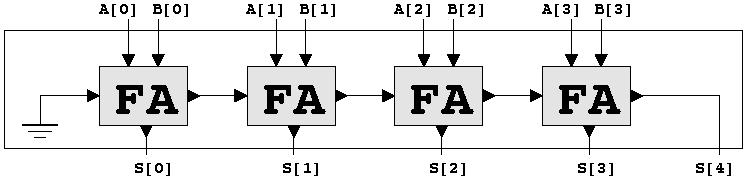
\includegraphics{adder.pdf}
  }
\caption{Addition of two integers (coded as bit vectors), using \emph{full adders}\label{binaryadder}}
\end{figure}

The following \alfa{} system describes a \emph{full adder}:
\index{full adder}
\begin{verbatim}
      system FullAdder (A,B,Cin : boolean) 
               returns (X,Cout : boolean);
      let
        X = A xor B xor Cin;
        Cout = (A and B) or (A and Cin) or (B and Cin);
      tel;
\end{verbatim}

To build an adder using this program, we need to 
instanciate a collection of such system,
as shown in Fig.\ref{binaryadder}. The shape of this collection may
be expressed as the {\alfa} domain \texttt{\{b|0<=b<W\}} where
\texttt{W} is a size parameter giving the number of bits of the
adder.
\index{use statement}

The \textbf{use} construct of {\alfa} allows precisely that: the
following system describes in {\alfa} the adder given in
figure~\ref{binaryadder}:
\index{adder}\index{binary addition}

\begin{verbatim}
system Plus: {W|W>1} (A,B: {b| 0<=b<W} of boolean)              -- 1       
             returns (S : {b| 0<=b<=W} of boolean);             -- 2       
var                                                             -- 3       
  Cin, Cout, X : {b| 0<=b<W} of boolean;                        -- 4       
let                                                             -- 5       
  Cin[b] =                                                      -- 6       
    case                                                        -- 7       
      {| b=0} : 0[];                                            -- 8       
      {| b>0} : Cout[b-1];                                      -- 9       
    esac;                                                       -- 10      
  use {b| 0<=b<W} FullAdder[] (A,B,Cin) returns(X, Cout);       -- 11      
  S[b] =                                                        -- 12      
    case                                                        -- 13      
      {| b<W} : X;                                              -- 14      
      {| b=W} : Cout[W-1];                                      -- 15      
    esac;                                                       -- 16      
tel;                                                            -- 17      
\end{verbatim}

\index{use statement}
In this system, line 11 reads as follows: 
\begin{quote}
``Use (or instantiate)
a collection of
instances of the subsystem \texttt{FullAdder}. This collection has the
shape of the extension domain\index{extension domain} \verb!{b| 0<=b<W}! and is thus indexed
by index \texttt{b}. Let the inputs of the \texttt{b}-th instance be
the variables \texttt{A}, \texttt{B} and \texttt{Cin} at point
\texttt{b}, and similarly let the outputs of this collection of
instances be the variables \texttt{X} and \texttt{Cout}.''
\end{quote}
Lines~6-10 describe the carry propagation, and lines~12-16
define the output of this binary adder.

\index{dimension extension}
In other words, line~11 is a shortcut for the following equations,
which are those of the system \texttt{FullAdder} whith the dimension
of the variables extended from zero to one:

\begin{verbatim}
        X[b] = A[b] xor B[b] xor Cin[b];
        Cout[b] = (A[b] and B[b]) or (A[b] and Cin[b]) or (B[b] and Cin[b]);
\end{verbatim}


\subsection{Syntax of the \emph{use} construct}

\index{use syntax}
The \textbf{use}\ construct appears at the syntactic level of an
equation, since it is basically a shortcut for a set of
equations. Here is the general syntax of an equation/use (see
appendix~\ref{alpha1} for the meta syntax):
{\tt
\begin{tabbing}
xxx\= xxx\= xxx\= xxx\= xxx\= xxx\= xxx\= xxx\= xxx\=  \kill
\textsl{Equation} ::=\\
\>\> \textsl{Identifier} = \textsl{Expression} ;\\
\> \Alt\ \> use \Opt{ \textsl{ExtensionDomain}} \textsl{Identifier}\\
\>\>\>\>\>\> \Opt{[\textsl{ParamAssignment} ]} \\
\>\>\>\>\>\>( \textsl{ExpressionList} )\\
\>\>\> returns\>\>\> ( \textsl{IdentifierList} ) ;
\end{tabbing}
}
 
\index{parameter assignation}\index{assignation of the
parameters}\index{parameters}
In this syntax we see that there is an optional \emph{parameter
assignment} which is discussed in the following.
In the previous addition the subsystem \texttt{FullAdder} has
no parameters, and the parameter assignment is therefore empty. 

\subsection{Manipulating structured programs}

A structured program is stored in {\mmalfa{}} as a {\mma{}} list of
systems called a \emph{library}. The default library is stored in the
global variable \verb!$library!.\index{$library}

A structured program may be written in one single file or several
distinct files.  In the former case the \texttt{load[]} function
returns a library composed of all the systems contained in the file,
and stores this library in \verb!$library!. %$ 

If the program is stored in several files, it is the responsability of
the user to build a proper library, i.e. a {\mmalfa{}} list of all the
systems needed by the hierarchical structure of the program. For this
purpose, the user will typically use {\mmalfa{}} list manipulating
functions such as \texttt{Join[], Append[]}, etc.\index{structured
programs}

In addition, two functions, \texttt{putSystem[]} and
\texttt{getSystem[]}, may be used to extract a system from a library
and to put back a modified system in a library. Typically a
system is extracted from the library as the {\em current}
system, modified by some program
transformation, and then put back in the library.\index{putSystem[]}\index{\getSystem[]}

\subsection{Program transformations associated with structures}

Most \mmalfa{} functions handle parameterized programs and \emph{use}
statements. There are, however, some major exceptions such as the
\texttt{writeC[]} translator \index{writeC[]} which generates code
only for flat {\Alpha} programs without subsystems. 
\mmalfa{}
provides functions to transform a structured program
into a ``flat'' equivalent one~:

\begin{itemize}
\item \texttt{assignParameterValue[]} \index{assignParameterValue[]}
gives a value to a size parameter, i.e. it refines a generic system
into a specialized one.
\item \texttt{inlineSubSystem[]} \index{inlineSubSystem[]} expands a
\emph{use} statement, replacing it with the equations of the
corresponding subsystem, properly modified to take the dimension
extension into account.\index{flattening a structured program}
\item \texttt{inlineAll[]} \index{inlineAll[]} recursively flattens a
structured {\alfa} program.
\end{itemize}
For more information see 
the subsystem documentation
\begin{verbatim}
$MMALPHA/doc/user/SubSystems.dvi
\end{verbatim}

\section*{Appendix: The polyhedral library}
\label{polylib}
See~\cite{Wilde93}(\texttt{http://www.irisa.fr/EXTERNE/bibli/pi/pi785.html}






% Introduction to Alpha, scalar part

% Based on DEA cours

\chapter{Modelling synchronous architectures}
\label{chapalphascal}

\begin{tobedone}
\begin{enumerate}
\item Redraw figures (after reinstalling X11 and xfig)
\end{enumerate}
\end{tobedone}

In this chapter, we present the {\alfa} language through the 
description of very simple -- and seemingly artificial -- examples
of synchronous circuits\index{synchronous circuits}. Our goal is to show the basic constructors
of the language: their syntax, their meaning, and how they can be
used in practice. 
% 
%\newpage
\section{Pointwise operators\index{pointwise operators}}
\begin{figure}[htbp]
%\htmlimage{scale=\myscale}
%\colorbox{white}{
\centerline{\includegraphics{figures/exemple_1}}
\caption{An adder\label{adder1}}
\end{figure}
Consider the architecture\index{architecture} shown in figure~\ref{adder1}: there is a 
simple adder\index{adder}, 
which takes to input flows, respectively {\tt x} and 
{\tt y}, and returns {\tt S}. 

This architecture is described by the {\alfa} program of figure \ref{adder-alpha}.
\begin{figure}[htbp]
%\htmlimage{scale=\myscale}
\verbatiminput{alpha_progs/adder.alpha}
\caption{An adder in {\alfa}}\label{adder-alpha}
\end{figure}
A program is called a {\em system}\index{system}. 
Line 1 is the head of the system, 
with name {\tt exemple1}. This system has two input arguments
named
{\tt x} and {\tt y}. These arguments, called {\em variables}\index{input
variables}, are
defined on the set {\tt \{t | 1 <= t\}}. Line 3 defines a local variable\index{local variable}
{\tt S} (for the moment, this variable is useless, but we shall
soon find a use for it). 
Between the {\tt let} and {\tt tel} keywords of lines 4 and
7, we have two equations\index{equation}: 
line 5 says that {\tt S} is the pointwise sum of 
{\tt x} and {\tt y}. In other words, $\forall t, S_t = x_t + y_t$. 
Line 6 says that {\tt z} and {\tt S} are identical.
\subsection*{Processing this example in {\mmalfa}}
Here are the Mathematica expressions that allow one to try
the previous example under MMAlpha.
%A more complete introduction to {\mmalfa} is given in 
%appendix~\ref{mma-introduction}.
\begin{verbatim}
load["adder.alpha"]    (* loads the alpha file *)
ashow[];               (* shows its content *)
\end{verbatim}

%
%\newpage
\section{Delays as dependence fonctions}
We now modify this example, by adding a delay\index{delay} on the output, as
shown in figure \ref{adderDelayed}. 
\begin{figure}[htbp]
%\htmlimage{scale=\myscale}
\centerline{\includegraphics{figures/exemple_2}}
\caption{Adder delayed}\label{adderDelayed}
\end{figure}
The corresponding {\alfa} program is shown in figure \ref{adderDelayed-alpha}.
\begin{figure}[htbp]
%\htmlimage{scale=\myscale}
\verbatiminput{alpha_progs/adderDelayed.alpha}
\caption{Adder plus delay}\label{adderDelayed-alpha}
\end{figure}
In this example, the definition domains\index{domain} of {\tt z} and {\tt S} have
changed: indeed, the output of the adder\index{adder (delayed)} is defined only one
cycle after the input. Thus, {\tt z} and {\tt S} are declared on 
domain {\tt \{t|2<=t\}}. Instruction 4 now defines {\tt S} as being the
sum of variables {\tt x+y}, delayed by 1. 

%
%\newpage
\section{Retiming\index{retiming}}
{\alfa} provides tools for retiming synchronous architectures. 
In the example of figure~\ref{adderDelayed}, one can shift the 
delay from the output of the adder to its inputs. 
This corresponds to replacing line 4 in program~\ref{adderDelayed-alpha}
by \verb\S[t] = x[t-1] + y[t-1];\. The corresponding architecture is shown 
in figure~\ref{adderRetimed}.
\begin{figure}[htbp]
%\htmlimage{scale=\myscale}
\centerline{\includegraphics{figures/exemple_3}}
\caption{Retiming the adder}\label{adderRetimed}
\end{figure}
\subsection*{Retiming in {\mmalfa}}
Do 
\begin{verbatim}
load["adderDelayed.alpha"]; (* load the alpha program *)
ashow[];                      (* show it *)
normalize[];                  (* simplify it *)
ashow[];                      (* show the result *)
asave["file.alpha"];          (* save program *)
\end{verbatim}

%
%\newpage
\section{Case and restrictions}
\begin{figure}[htbp]
%\htmlimage{scale=\myscale}
\centerline{\includegraphics{figures/exemple_5}}
\caption{Adding a multiplexer}\label{adderMultiplexer}
\end{figure}

Two other constructs of the language are the case\index{case} and the
restriction.  Consider the example of figure~\ref{adderMultiplexer},
which shows a new delayed and retimed version of the adder, where the
output is taken through a multiplexer\index{multiplexer}. In other
words, depending on the value of index {\tt t}, {\tt S} is either 0 or
the sum {\tt x[t-1] + y[t-1]}. This is reflected in the definition of
{\tt S} in figure~\ref{addermultiplexer-alpha} (lines 2--5.) This
definition uses a case expression. Each branch\index{branch (of a case
expression)} of the case is an {\alfa} expression. The first one is
the constant\index{constant} $0$, denoted as {\tt 0[]} in {\alfa}. It is
considered only when {\tt t} is equal to $1$, which is reflected in the
condition\index{condition} {\tt \{| t = 1\}}. The second branch
corresponds to the expression {\tt x[t] + y[t]}, taken when the
condition {\tt \{|t>1\}} is true. Actually, we call an expression such
as {\tt \{|t>1\}} a {\em restriction}.\index{restriction}

\begin{figure}[htbp]
%\htmlimage{scale=\myscale}
\verbatiminput{alpha_progs/adderMultiplexer.alpha}
\caption{Adder and multiplexer}\label{addermultiplexer-alpha}
\end{figure}
The definition of {\tt z} also uses a restriction. The definition of 
line 6 says that {\tt z} is defined as {\tt S}, but only for time 
instants {\tt t} such that {\tt \{|t>=5\}}. 
\subsection*{Exercices in {\mma}}
Load and parse program adderMultiplexer.alpha.
\begin{verbatim}
load[adderMultiplexer.alpha];
ashow[adderMultiplexer];
\end{verbatim}

%
%\newpage
\section{Array and full form of {\alfa}}
\label{arrayform}

In all the above examples, we have used the so called {\em array
form}\index{array form} of {\alfa}. The full form\index{full form} of
the language is actually a little bit different, and a little bit more
difficult to read initially. It is however needed in order to
understand some of the properties of the language.

Let us consider again the definition of {\tt S} in
program~\ref{addermultiplexer-alpha}, line 2 -- 5:
\begin{verbatim}
 S[t] = case
     {|t=1}: 0[];
     {|t>1}: x[t-1] + y[t-1];
     esac;
\end{verbatim}
The full form of this expression is in fact: 
\begin{verbatim}
 S = case
      {t|t=1}: 0.(t->);
      {t|t>1}: x.(t->t-1) + y.(t->t-1);
  esac;
\end{verbatim}
To explain this, we need to go more deeply in the 
structure of the language. In {\alfa}, any expression is a function from
a set of points -- called the {\em domain} of the expression --, 
to some value set depending on the type of the expression. 
Expressions are either 
\begin{itemize}
\item variables -- e.g. {\tt S},\index{variables} 
\item scalar constants\index{constants}
\item pointwise operations on expressions -- e.g. {\tt x + y}\index{pointwise 
operators}
\item application of dependence functions to expressions, -- e.g. 
{\tt exp.f} where {\tt f} is a dependence function explained later,\index{dependence function}
\item restriction of expressions, -- e.g. {\tt dom: exp}, where 
{\tt dom} is a domain description\index{restriction},
\item case expressions -- e.g. {\tt case e1 ; e2; esac}, where {\tt e1}
and {\tt e2} are expressions.\index{case expression}
\end{itemize}

Let us examine expressions in more details. 
\subsection{Domains}
\index{domain}

Domains of {\alfa} are restricted to {\em polyhedra}, (more precisely,
unions of finitely may polyhedra).  A polyhedron is a set of integral
points whose coordinate satisfy linear inequalities.  For example:
{\tt \{t | 1 <= t <= 10\}} denotes such a set. So also does {\tt \{i,j
| i>=10; 0 <= j <= i\}} for example. {\texttt \{i | 0 < i < 10\} ||
\{i | 15 <= i\}} is a union of polyhedra.  \index{polyhedron}

\subsection{Variables}
\index{variable}
Variables are functions from a domain to a set of values. For example, 
in program~\ref{addermultiplexer-alpha}, {\tt S} is a function from 
the domain {\tt \{t|1<=t\}} to the set of integers. Thus, {\tt S}
represents a collection of indexed values $S_t$, where {\it t} belongs
to the domain of {\tt S}. 

{\alfa} is a strongly-typed language, where variables are declared,
together with their domain. This allows many compile time checks to be
performed\index{type-checking} (see chapter~\ref{chapanalyze}).

Input variables are defined in the head of the system
definition. Output variables are defined after the key-word {\tt
result}. Local variables are defined after the key-word {\texttt var}
and the keyword {\tt let}.

\subsection{Constants}
In {\alfa}, constants are considered as functions from the
singleton set $Z^0$ to a type. For example, $1$ is the function 
from $Z^0$ to the integer value $1$. 
\subsection{Pointwise operations}
\index{pointwise operations}

Pointwise operations generalize classical operations like +, -, * on
integers, or {\tt and}, {\tt not}, {\tt or} on booleans. So, {\tt x +
y} represents the pointwise operation on values $x_t$ and $y_t$ for
all $t$. There is however, an important point to notice: if {\tt op}
is a pointwise operator and {\tt e1} and {\tt e2} are expressions,
then the domain of the expression {\tt e1 op e2} is the {intersection}
of the domains of {\tt e1} and {\tt e2}.\index{domain of a pointwise
expression}

\subsection{Dependence functions}
\index{dependence function}

Dependence functions are affine functions on indices.
They are denoted as
\begin{center}
\texttt{(idx, idx, ... -> iexp, iexp, ... )}
\end{center}
where \texttt{idx} is an index name and \texttt{iexp} is an affine
function of indices.  For example: {\tt (i,j -> i+2, j+3i-4)\}}
denotes such a function.  So does also the function {\tt f=(t ->
t-1)}. Therefore, {\tt x.(t -> t-1)} is an {\alfa} expression, whose
meaning is as follows.  Remember that {\tt x} is a function from the
domain {\tt \{t | 1<=t\}} to the set of integers. The composition of
functions {\tt x o f} is therefore defined, and this is just what {\tt
x.(t -> t-1)} represents. It is easy to see that this function is
defined on the domain {\tt \{t | t>=2\}}.  More generally, the domain
of any expression {\tt e.f} is ${\tt f}^{-1}(\mbox{dom}({\tt e}))$,
that is to say, the pre-image of the domain of {\tt e} by function
{\tt f}.

Note that a function {\tt (->t)} denotes a mapping from the set $Z^0$
to $Z$. Similarly, {\tt (t ->)} denotes a mapping from the set $Z$ to
$Z^0$. Such functions are used to extend scalar constants to higher
dimensional domains.\index{Extension of constants}

\subsection{Restriction expressions}

\index{restriction} As said before, restrictions allows one to
restrict the definition of an expression to a subdomain. To be
consistent with the other language constructs, restrictions are
defined as polyhedra, and therefore are denoted just as domains. For
example, {\tt \{t | t>=5\}: S} is a restriction of the expression
\texttt{S} to domain \texttt{\{t | t >= 5\}}. The domain of a
restricted expression \texttt{dom: e} is the intersection of the
domain of the expression and the domain defined by the restriction,
i.e., $\texttt{dom} \cap \texttt{e}$.\index{domain of a restriction}

\subsection{Case expressions}

\index{case expression} As already seen, case expressions allow one to
define a new function case by case. A case expression is defined on
the union of the domains of its branch. Let {\tt case exp1; exp2 esac}
be a case expression, with branches {\tt exp1} and {\tt exp2}. Let
{\tt d1} and {\tt d2} be respectively the domains of {\tt exp1} and
{\tt exp2}. Assume that {\tt d1} and {\tt d2} have the same
dimensionality and are disjoint (these properties are checked during
static analysis). Assume also that {\tt exp1} and {\tt exp2} have the
same type, say {\tt T}.  Then {\tt case exp1; exp2 esac} is a function
from ${\tt d1} \cup {\tt d2}$ to {\tt T}, whose value is that of {\tt
exp1} on {\tt d1}, and that of {\tt exp2} on domain {\tt d2}. For 
a detailed desciption of the domain computations and its use for the
static analysis, see section~\ref{static-analysis}.

\subsection*{Back to our example}
We are now ready to consider again the example corresponding to figure~\ref{addermultiplexer-alpha}. The definition of {\tt S} is:
\begin{verbatim}
 S = case
      {t|t=1}: 0.(t->);
      {t|t>1}: x.(t->t-1) + y.(t->t-1);
  esac;
\end{verbatim}
Let us analyze each branch. {\tt 0} is a function from $Z^0$ to 
the integer value $0$. Composing this function with the function 
\texttt{(t ->} extends the constant {\tt 0} to the set $Z$. In other 
words, {\tt 0.(t->)} denotes the function from $Z$ to integers,
whose value is {\tt 0} everywhere. 
{\tt \{t | t=1\}: 0.(t->)} denotes the restriction of this function 
to the single point {\tt t=1} of $Z$. 

We can analyze the second branch in a similar fashion. We would conclude
that it represents a function from the subset {\tt \{t | t>1\}} of $Z$, 
whose value at point {\tt t} is $x_{t-1} + y_{t-1}$. 

Finally, the total case expression defines {\tt S} as a function from
{\tt \{t | t >=1\}} to the integer set, whose value is {\tt 0} 
when {\tt t = 1}, $x_{t-1}+ y_{t-1}$ otherwise.

\subsection{Array form}
\index{array form}

The array form is just a convenient way of presenting {\alfa} programs, 
in a more ``readable'' form. The rule is simple to explain on the 
definition of {\tt S}:
\begin{itemize}
\item Dependence functions of the form {\tt .(indices -> exprs)} are rewritten
as {\tt [exprs]}, 
\item Restrictions of the form {\tt \{indices | inequalities\}} are rewritten
{\tt \{| inequalities\}},
\item Left-hand side variables are appended with the indices from the
right hand side.
\end{itemize}
Thus, the definition of {\tt S} in array form is
\begin{verbatim}
 S[t] = case
      {|t=1}: 0[];
      {|t>1}: x[t-1] + y[t-1];
  esac;
\end{verbatim}
This notation can be used safely for any normalized expression, as 
we shall see in section~\ref{substitution}.
\subsection*{Exercices in {\mmalfa}}
Load a program, and see its full form using the {\tt show[]}
function, or its array form using {\tt ashow[]}.
%\newpage
\section{Substitution and normalization}
\label{substitution}
One of the properties of {\alfa} is called the referential transparency\,:
\index{referential transparency}
it means that the meaning of an expression is independent of the context
where it appears. 
For this reason, any symbol can be safely replaced by its definition. 
For example, by replacing the {\tt S} symbol in the definition of 
{\tt z} in program~\ref{addermultiplexer-alpha}, we obtain the 
program shown in figure~\ref{addermultiplexer-alpha}.
\begin{figure}[htbp]
%\htmlimage{scale=\myscale}
\verbatiminput{alpha_progs/adderSubstituted.alpha}
\caption{Program of figure~\ref{addermultiplexer-alpha} after substitution of {\tt S} in 
definition of {\tt z}}\label{addersubstituted-alpha}
\end{figure}



Let us consider the new definition of {\tt z}:
\begin{verbatim}
z = {t | 5<=t} : 
         case
           {t | t=1} : 0.(t->);
           {t | 2<=t} : x.(t->t-1) + y.(t->t-1);
         esac.(t->t);
\end{verbatim}

\begin{figure}[htbp]
%\htmlimage{scale=\myscale}
\verbatiminput{alpha_progs/adderNormalized.alpha}
\caption{Normalization of program~\ref{addersubstituted-alpha} (in
array form)}
\label{addernormalized-alpha}
\end{figure}

It is rather intuitive that the first restriction {\tt \{t | 5<=t\}}
can be distributed in the branches of the case expression. Combining
(i.e., intersecting) this restriction with the {\tt \{t | t=1\}} leads
obviously to an empty set, and consequently, to an empty
branch. Similarly, combining {\tt \{t | 5<=t\}} with {\tt \{t | 2<=t\}}
leads to {\tt \{t | 5<=t\}}. In summary, we can imagine that the full
definition of {\tt z} can be simplified to something like {\tt z =
x.(t->t-1) + y.(t->t-1)}.

\begin{figure}[htbp]
%\htmlimage{scale=\myscale}
\centerline{\includegraphics{figures/exemple_7}}
\caption{Architecture after substitution and normalization}
\label{addernormalized}
\end{figure}
These intuitive properties are in fact true, and such a simplification
is done in a systematic way by means of the normalization
transformation: one can prove that any expression can be simplified
into a normalized one, with at most one level of outermost case, one
level of restrictions, and one level of
dependences.\index{normalization}\index{simplification of expressions}

After normalization, the program becomes that of
figure~\ref{addernormalized-alpha}.

We can interpret this program as representing the synchronous
architecture of figure~\ref{addernormalized}.
We can see -- and this is of course straightforward -- that the 
multiplexer is indeed useless, since we are interested in the 
value of {\tt z} only when {\tt t>1}. This normalization 
property is one of the most important one of {\alfa}. 

\subsection*{Exercices in {\mma}}
\subsubsection*{Exercice 1}
Write an {\alfa} program to model the 
following
architecture:
%of figure~\ref{exo1}.
\begin{figure}[htbp]
%\htmlimage{scale=\myscale}
\centerline{\includegraphics{figures/exo1}}
\caption{Exercice 1}
\label{exo1}
\end{figure}
\subsubsection*{Exercice 2}
Write an {\alfa} program to model 
the circuit of figure~\ref{exo2}.
\begin{figure}[htbp]
%\htmlimage{scale=\myscale}
\centerline{\includegraphics{figures/exo2}}
\caption{Exercice 2}\label{exo2}
\end{figure}




% Introduction to Alpha, array part

% Based on DEA cours

\chapter{Arrays of synchronous operators}
\label{chapalphaarray}
In this chapter, we show how arrays of hardware operators can be modelled in
{\alfa}\index{arrays}. In chapter~\ref{chapalphascal}, the basic
operators of the language were described. As we shall see here, a 
simple extension of these operators allows two-dimensional -- and
higher-dimensional -- variables and expressions to be used. 

\section{Describing array of elements}
Figure~\ref{adder-array} shows an array of adders. 
\section{An array of adders}
\begin{figure}[htbp]
%\htmlimage{scale=\myscale}
%\colorbox{white}{
\centerline{\includegraphics{figures/exemple_9}}
%}
\caption{An array of adders}\label{adder-array}
\end{figure}

The corresponding {\alfa} code is shown on figure~\ref{adder-array-alpha}.
\begin{figure}[htbp]
%\htmlimage{scale=\myscale}
\verbatiminput{alpha_progs/adder-array.alpha}
\caption{An array of adders in {\alfa}}\label{adder-array-alpha}
\end{figure}
Blabla
\section{Change of basis}
Any {\alfa} program can be seen as a black box which takes input
variables, and produces output variables. Therefore, intermediate
variables are unimportant, and, in particular, one can reindex them
using one-to-one index mappings. Obviously, 
\begin{verbatim}
A[i] = B[i];
B[i] = C[i];
\end{verbatim}
is identical to 
\begin{verbatim}
A[i] = B[i-1];
B[i] = C[i+1];
\end{verbatim}
 The change of basis operation does just this reindexing. In the
context of {\alfa}, the reindexing functions that we consider need to
be restricted to affine {\em unimodular functions},\index{affine
functions}\index{unimodular functions} that is to say, affine mappings
which admit an integral inverse.

Consider variable {\tt Z} in program~\ref{adder-array-alpha}. Consider
the reindexing function $B$ from $\Z^2$ to itself, defined by $B(t,p)
= (t+p,p)$. One can show that $B$ is unimodular. Let us denote
$B$ using the {\alfa} syntax, as {\tt (t,p -> t+p,p)}. This function 
is one-to-one, and its inverse is $B^{-1}$, denoted {\tt (t,p -> t-p,p)}.

To apply the change of basis defined by $B$ on variable {\tt Z}, 
we need to do the following operations:
\begin{enumerate}
\item Replace the domain of definition of {\tt Z} by its image under
the $B$ mapping. As the domain of {\tt Z} is 
{\tt \{t,p|t>=1;4>=p;p>=0\}}, its image by $B$ is 
{\tt \{t,p | p+1<=t; 0<=p<=4\}}.
\item Replace any occurrence of {\tt Z} in a right-hand side of 
an equation by {\tt Z.(t,p -> t+p,p)}.
\item Replace the entire equation {\tt Z = expr} defining {\tt Z}
by {\tt Z = expr.(t,p -> t-p,p)}.
\end{enumerate}

The new program is shown in figure~\ref{adder-array-bn-alpha}. We can normalize
it, which leads to program~\ref{adder-array-cb-alpha}.
\begin{figure}[htbp]
%\htmlimage{scale=\myscale}
\verbatiminput{alpha_progs/adder-array-bn.alpha}
\caption{Program adderarray, after change of basis {\tt (t,p->t+p,p)}
performed on {\tt Z}}\label{adder-array-bn-alpha}
\end{figure}

This new program can be interpreted as the architecture shown in 
figure~\ref{adder-array-cb-tex}.
\begin{figure}[htbp]
%\htmlimage{scale=\myscale}
\verbatiminput{alpha_progs/adder-array-cb.alpha}
\caption{Program adderarray, after change of basis 
and normalization}\label{adder-array-cb-alpha}
\end{figure}

\begin{figure}[htbp]
%\htmlimage{scale=\myscale}
%\colorbox{white}{
\centerline{\includegraphics{figures/exemple_10}}
%}
\caption{An array of adders}\label{adder-array-cb-tex}
\end{figure}

% Reduction
%\centerline{\input{/udd/quinton/documents/lncs_574/seminaire_litp/figures/exemple_8}}
%\input{/udd/quinton/documents/lncs_574/seminaire_litp/exemples_alpha/exemple_8}
%
%\transparent{0cm}{{Convolution}}{0cm}
%{\small
%\input{/udd/quinton/cours/cours_nouveau/convgen}
%}
%\transparent{0cm}{{Convolution apr\`{e}s s\'{e}rialisation}}{0cm}
%{\small
%\input{/udd/quinton/cours/cours_nouveau/conv}
%}
%\transparent{0cm}{{Convolution, apr\`{e}s changement de base}}{0cm}
%{\small
%\input{/udd/quinton/cours/cours_nouveau/conv1}
%}
%\begin{slide}{}
%\titre{Conception typique (Mathematica Alpha)}
%{\small
%\begin{enumerate}
%\item Analyse syntaxique, v\'{e}rification
%\item Placement des variables (manuel)
%\item Uniformisation (automatique)
%\item Ordonnancement (automatique)
%\item Changement  de base (automatique)
%\item Separation espace et temps
%\item Remplacement des {\bf case} par des signaux de contr\^{o}le (automatique)
%\item Generation circuit (MadMacs ou VHDL) 
%\end{enumerate}
%}
%\end{slide}




\subsection*{Processing this example in {\mmalfa}}
Load the array of adders:
\begin{verbatim}
load["adder-array.alpha"];   (* loads the alpha file *)
ashow[];                     (* shows its content *)
\end{verbatim}
Apply a change of basis:
\begin{verbatim}
changeOfBasis["B.(t,p->t+p,p)"];  (* apply a change of basis *)
ashow[];                     (* shows the result *)
\end{verbatim}
Notice that the result of a change of basis is automatically normalized. 

\section{Conclusion}
In this chapter, we have seen how arrays of elements can be 
described using {\alfa}. In order to present hardware examples, we
have limited ourself to programs where the indexes can be
interpreted as the time and the space (i.e., {\tt t} and {\tt p}).
Actually, {\alfa} programs are not restricted to such indexes. 
{\em Au contraire}, hardware-like {\alfa} programs represent the 
ultimate goal of a synthesis process which starts from a 
behavioural specification. They are in fact a proper subset of all 
{\alfa} programs.

In Chapter~\ref{chapfunctional}, we shall consider {\alfa} from the
data parallel perspective. 



% Introduction to Alpha, a la Sanjay! 

\chapter{The Alpha Language and System -- Another point of view}
\label{chapfunctional}
\section{Introduction}

\begin{tobedone}
The last figure is garbage. The psfig inside has been commented out. 
See reference document in old pdf turorial.
\end{tobedone}
Alpha is a functional language, based on recurrence
equations\index{recurrence equation}.  All variables are type-declared
at the beginning of a program, and represent multidimensional arrays,
whose shapes can be arbitrary polyhedra.  For example, the declaration
\verb!A: {i,j| 0<j<i<=N} of real!, specifies a (strictly) lower
triangular, real matrix\index{lower triangular linear system}.  To
introduce the main features of the language, consider the problem of
solving a system of linear inequalities, $Ax=b$, where $A$ is a lower
triangular, $n\times n$ matrix with unit diagonal.  It is well known
that this can be solved using forward substitution\index{forward
substitution}, as given by the following formula.  \[\mbox{for } i =
1\ldots n,~~x_i = b_i - \sum_{j=1}^{i-1} A_{i,j} x_j\]

\begin{figure}[tb]
%\htmlimage{scale=\myscale}
\setlength{\unitlength}{10mm}
\begin{center}
%\begin{picture}(16,2.5)
%\thicklines
%\put(-0.1,-0.7){\framebox(16.2,3.7){}}
%\begin{boxedminipage}[b]{16cm}
%{\footnotesize
\begin{verbatim}
system ForwardSubstitution : { N | N>1 }       -- comments are like this
                 ( A : { i,j | 0<j<i<=N } of real;    -- a 2D input variable
                   B : { i   | 0<i<=N } of real)      -- a 1D input variable
         returns ( X : { i   | 0<i<=N } of real );    -- a 1D output variable
  let
    X[i] = B[i] - reduce(+, (i,j -> i), A * X.(i,j->j))[i]
  tel;
\end{verbatim}
%\end{boxedminipage}
%\end{picture}
\end{center}
%\vspace*{-0.8cm}
\caption{Alpha program for the forward substitution algorithm}
\label{fig-fs}
\end{figure}

  The corresponding Alpha program (Fig.~\ref{fig-fs}) is identical, except for
syntactic sugar.  The first line names the system and declares that it has a
positive integer parameter, {\tt N}.  The next three lines are declarations of
the input and output variables of the system.  Note how each variable is
defined over a certain range of indices, specified by a set of linear
inequalities.  This defines a polyhedron, called its {\em domain}.  For
example, the domain of {\tt A} is triangular, while {\tt B} and {\tt X} are
one dimensional vectors.  Variables declared before the ``{\tt returns}''
keyword are input variables, and those after it are outputs.  Although our
example does not illustrate it, a system may also have local variables, which
are declared after the system header, using the keyword {\tt var}.  The body
of the program is a number of equations delineated by the {\tt let} and {\tt
tel} keywords.  Here, we have a single equation corresponding to the above
formula, which specifies that we compute {\tt X[i]} by performing a reduction
(any associative and commutative binary operator may be used; here we have
{\tt +}).  The {\tt (i,j->i)} specifies a projection of a two dimensional
index space to one dimension.  Intuitively, it states that within the body of
the {\tt reduce}, we have two index variables, {\tt i} and {\tt j}, but the
latter is not visible outside the scope of the {\tt reduce}.  The body of the
{\tt reduce} is the expression, {\tt A * X.(i,j->j)}, where {\tt (i,j->j)}, is
a {\em dependency}. It denotes the fact that to compute the body at index
point, {\tt [i,j]}, we need the value of {\tt X} at index point {\tt j} (the
dependency of {\tt A} is not explicitly written---it is the identity).
Dependencies are an important aspect of Alpha.  They describe ``indexing
functions'' and have the syntax,
 \verb! (idx, idx, ...  -> i-expr, i-expr, ...)!, where each {\tt idx} is an
index name, and {\tt i-expr} is an {\em affine} expression of the system
parameters and the {\tt idx}'s.  The Alpha system uses this syntax for
specifying a multidimensional affine function in many different contexts.

\section{Polyhedra and affine functions}
  Alpha imposes the restriction that all variable domains are polyhedral, and
all dependencies are {\em affine} functions.  Although this may constrain our
expressive power, it is a conscious choice that was made for many reasons.  A
large number of linear algebra and DSP and image processing algorithms fall
within these limitations.  It is also known 
%\cite{feautrier91}, 
that any
nested loop program (in a conventional language) that satisfies certain
constraints (loop bounds are affine functions of the parameters and outer
indices, and the body contains only assignments to array variables which are
accessed using only affine functions of the loop indices) can be modeled by a
formalism that is similar to an Alpha program.  Such assumptions are made in
many techniques used in parallelizing compilers.  By concentrating explicitly
on this subset of programs, we can make use of powerful static analysis and
optimization tools based on polyhedra and linear programming (implemented in
our {\bf polyhedral library}.
%\cite{wilde93-poly}).  
Finally, it is precisely
these restrictions that interact coherently and form the foundation of our
transformational system.  They also ensure that all Alpha programs can be put
into a ``normal'' form, and in fact, all examples that we use here have been
so normalized.

\section{Transformations in Alpha}

  We now introduce some of the Alpha transformations used in converting our
program into a single assignment C program.  
\subsection{Serialization}
The first one is used to {\bf
serialize} the reduction operation, and requires two parameters: the
``direction'' in which we accumulate the partial sums, and the name of the
temporary variable.  For our example, if we choose to accumulate in the {\em
increasing} direction of {\tt j} (specified as ``{\tt (i,j->i,j+1)}'') and
name the new variable, {\tt f}, we obtain the Alpha program shown in
Fig.~\ref{fig-serial}.  We also see two new syntactic constructs, the {\em
case} (which has the usual meaning), and the {\em restrict}, which has the
syntax,
 \verb!<polyhedron>: <expr>!, and denotes the expression, {\tt <expr>} but
restricted to the subset of index points in {\tt <polyhedron>}.

  Observe that the domain of {\tt f} is \verb!{i,j| 0<=j<i; 2<=i<=N}! (a
``nearly triangular'' trapezium defined by the points {\tt [2,0]} {\tt [2,1]}
{\tt [N,N-1]} and {\tt [N,0]}).  Also note that the equation for {\tt X} now
has the expression {\tt f[i,i-1]} replacing the reduction, and the new
equation for {\tt f} consists of an initialization at the boundary, and an
accumulation using the {\em body of the original reduction}.  All this is
automatically determined by the system, using the polyhedral library.

\begin{figure}[tb]
%\htmlimage{scale=\myscale}
\setlength{\unitlength}{10mm}
\begin{center}
\begin{picture}(16,5.7)
\thicklines
\put(-0.1,-0.7){\framebox(16.2,6.7){}}
\put(11,0.5){\framebox{The domain of {\tt f}.}}
\put(11,1.3){\begin{picture}(6,3)
              \put(0,0){\includegraphics{figures/domain-f.pdf}}
              \put(-0.3,3.2){$i$}
              \put(0.5,3.6){$j$}
              \put(-1,2.7){\small\tt [2,0]}
              \put(1,2.7){\small\tt [2,1]}
              \put(-1,0){\small\tt [N,0]}
              \put(3.4,0){\small\tt [N,N-1]}
              \end{picture}}
\begin{boxedminipage}[b]{16cm}
\hspace*{2cm}$\vdots$\small
\begin{verbatim}
var
  f : {i,j | (2,j+1)<=i<=N; 0<=j} of real;
let
  f[i,j] = case
        {| j=0} : 0[];
        {| 1<=j} : f[i,j-1] + A * X[j];
           esac;
  X[i] = case
        {| 2<=i} : B[i] - f[i,i-1];
        {| i=1} : B[i];
         esac;
tel;
\end{verbatim}
\end{boxedminipage}
\end{picture}
\end{center}
\vspace*{-0.8cm}
\caption{The forward substitution program after serialization}
\label{fig-serial}
\end{figure}

\subsection{Change of basis}
  Perhaps the most important transformation in the Alpha system is the {\bf
change of basis}.  The intuition behind it is as follows.  Since an Alpha
variable can be viewed as a multidimensional array defined over a polyhedral
domain, we should be able to ``move'' (or otherwise change the ``shape'' of)
its domain and construct an equivalent program.  For example, suppose we want
to rotate the domain of {\tt f} in Fig.~\ref{fig-serial} counterclockwise
by $45^\circ$, i.e., we desire to map the point {\tt [1,0]} to {\tt [1,1]},
and {\tt [1,1]} to {\tt [0,1]} (this makes a vertical line diagonal, and a
diagonal one horizontal).  It is easy to verify that the mapping
 \verb!(i,j -> i-j,i)! achieves this; the resulting program and transformed
domain are shown in Fig.~\ref{fig-transf} (the changes are highlighted).  In
general, when variable {\tt V} is transformed, the system must determine: (i)
its new domain, (ii) the new case structure of its equation, (iii) the new
dependencies for the uses of {\em all} variables in the equation for {\tt V},
and (iv) the new dependencies for {\em uses} of {\tt V} (in all other
equations).  All of this is done automatically using the polyhedral library,
and relies on the fact that the language allows a coherent interaction among
the domains, the dependencies and the (normal form) structure of the programs.

\begin{figure}[tb]
%\htmlimage{scale=\myscale}
\setlength{\unitlength}{10mm}
\begin{center}
\begin{picture}(16,5)
\thicklines
\put(-0.1,-0.7){\framebox(16.2,6.3){}}
%\put(3.4,4.5){\oval(4.7,0.5)}
%\put(2.5,3){\oval(2.2,0.9)}
%\put(6.9,2.8){\oval(5.9,0.5)}
%\put(5.5,1.55){\oval(1.4,0.5)}
\put(11,1){\begin{picture}(6,3)
             \put(0,0){\includegraphics{figures/rot-f}}
             \put(-0.3,3){$i$}
             \put(0.5,3.6){$j$}
             \put(0.3,2.3){\small\tt [2,2]}
             \put(0.8,3.5){\small\tt [1,2]}
             \put(3,3.5){\small\tt [0,N]}
             \put(2.5,-0.3){\small\tt [N,N]}
              \end{picture}}
\begin{minipage}[b]{16cm}
\hspace*{2cm}$\vdots$\small
\begin{verbatim}
  f : {i,j | 1<=i<=j; 2<=j<=N} of real;
let
  f[i,j] = case
        {| i=j}    : 0[];
        {| i<=j-1} : f[i+1,j] + A[j,-i+j] * X[-i+j];
           esac;
  X[i] = case
        {| 2<=i} : B[i] - f[1,i];
        {| i=1} : B[i] - 0[];
         esac;
tel;
\end{verbatim}
\end{minipage}
\end{picture}
\end{center}
\vspace*{-0.8cm}
\caption{The transformed program and the new domain of {\tt f}}
\label{fig-transf}
\end{figure}

The syntax for the affine mapping in a change of basis
transformation is the same as for dependencies, but there is a subtle
difference.  We should be able to transform the variable in any
(affine) manner, but we must always ensure that the {\em number} of
index points remains invariant.  For this, the affine change of basis
must admit an integral inverse (i.e., be {\em unimodular}).  We have
also developed a {\em generalized change of basis}, which allows
``non-square'' mappings (non-unimodular transformations are encoded as
a special case of this).






% Systolic array design

\chapter{Deriving \index{systolic}systolic architectures using {\alfa}}
\label{chapderiving}

{\sc Version of \today}

In this chapter, we describe a methodology for deriving
systolic architectures using {\mmalfa}. This \index{design
methodology}methodology is illustrated by means of an {\alfa}
program for the matrix-vector multiplication. A companion
notebook called \texttt{matvect.nb} allows the reader to
execute interactively this demonstration. This notebook is
situated in directory:\\
\texttt{\$MMALPHA/demos/NOTEBOOKS/Matvect}\\
A link to this notebook is available in the 
master notebook (see~\ref{master}).

\section{Introduction}

The methodology presented here is inherited from the research of the
``systolic community''~\cite{Meg1,KungHT,QuintonRo89} and from its
adaptation to {\alfa}~\cite{SieWilde94,Dinechin96c,Patricia96}.

The successive steps of the derivation are the following ones:
\begin{enumerate}
\item High level specification in {\alfa}.
\item Uniformization.
\item Scheduling and mapping.
\item Control signal generation.
\item \label{step5} Generation of an {\alphard} specification. 	\\
~\\These steps may be followed by three additional ones: 
\item Translation to {\vhdl}.
\item Logic synthesis.
\item Layout synthesis.
\end{enumerate}

The five first transformations deal with producing a so-called
\alphard{} program.  {\alphard} is a subset of the {\alfa} language
used for architectural description at the register transfer level.
The description of {\alphard} format can be found
in~\cite{Patricia96}, and is presented in chapter~\ref{chapvhdl}.  In
the present chapter, we only describe how to perform the first four above
steps using {\mmalfa}. The result will be a single {\alfa}
program which can be interpreted as a systolic array for executing the
original {\alfa} specification. The main difference between this
format -- called {\alphaz} -- and {\alphard} is their structuring: an
{\alphard} program is structured into several sub-systems while an
{\alphaz} program contains only one {\alfa} system.

\section{Example of the matrix-vector product\index{matrix-vector product}}
We start by an \alfa{} description of the algorithm, 
as shown in figure~\ref{figder1}. 

\begin{figure}[htbp]
%\htmlimage{scale=\myscale}
\verbatiminput{alpha_progs/MatVect.alpha}
\caption{{\alfa} program for the matrix-vector}
\label{figder1}
\end{figure}

The dependence graph of this program 
is shown in the left hand side of figure~\ref{figder2}, 
for $N=M=4$. In this
figure, it can be seen that each component of the {\tt b} vectors is
broadcasted to several computations. For instance, $b_1$ is used in
the computation of $ a_{1,1}, a_{1,2}, a_{1,3}$ and $a_{1,4}$. The
first step of the synthesis consists of ``pipelining'' these values
in order to obtain a uniform dependence graph such as 
that shown in the right hand side of
figure~\ref{figder2}. This step is often called {\em uniformization}
or {\em localization}
in the litterature.

\subsection{Uniformization\index{Uniformization}}

Methodologies for automatic uniformization were
proposed by several researchers
(see~\cite{QuintonVa88} for example). However, performing the
uniformization process completely automatically is difficult as there
are many possibilities for uniformizing a given program. Hence, 
this transformation requires some help from the user.

Before proceeding, we first perform a pre-processing 
transformation, which consists of adding a local 
variable \texttt{A} to replace the occurrence of
\texttt{a} in the definition of \texttt{C}. The purpose of
this modification is to anticipate a change of basis 
that will be done later on, and which cannot be applied on
an input variable without altering the semantics of
the program. The \mmalfa{} function which does this
is:\\
\texttt{addLocal["A = a"];}\\
%We first perform a single pre-processing step which consists of adding all
%the constraints present in the parameter domain declaration (present
%at the top of the system) inside every domain appearing in the
%program. Then we add, for each input variable, a local variable
%(remember that we cannot perform transformations involving inputs and
%output variables). Next, we have to \index{pipeline}pipeline the
%broadcasted expressions.

We are now ready to uniformize the occurence \texttt{b[i]}
in the definition of \texttt{C}. 
The pipeline vector will be the direction of
the $\vec{\imath}$ axis in our example, as shown in 
figure~\ref{figder2}.

\begin{figure}[htbp]
%\htmlimage{scale=\myscale}
\centerline{\includegraphics{figures/tr1}}
\caption{Dependence graph for the program of figure~\ref{figder1}, before 
and after uniformization.}
\label{figder2}
\end{figure}

In our example, the {\mmalfa} function for uniformizing is: 
\begin{verbatim}
pipeall["C","b.(i,j->j)","B1.(i,j->i+1,j)"];
\end{verbatim}
The parameters given to 
{\tt pipeall} can be read as follows: 
\begin{quote}
In the definition of {\tt C},
pipeline the expression
{\tt  b.(i,j->j)}. The pipeline vector is
$(1,0)$, the variable which will pipeline the value will be called
{\tt B1}.
\end{quote}
Two remarks: 
\begin{itemize}
\item The array notation {\tt b[i]} cannot be used
here, as it would be ambiguous. 
\item The pipeline vector is indicated as a translation in
{\alfa} form.  
\end{itemize}
The result of applying these commands is shown in
figure~\ref{figder3} where only the equation of the resulting {\alfa}
program are shown.  Note that the domains of the branches
of \texttt{B1} definition have been computed by {\tt
pipeall}. Note also that the dependence graph of this program
-- represented in the right hand side of figure~\ref{figder2} -- is
now uniform. For more information on the pipelining process refer
to the
documentation~\cite{docpipeline}.

\begin{figure}[htbp]
%\htmlimage{scale=\myscale}
\begin{verbatim}
B1[i,j] = 
      case
        {| i=1; 1<=j<=M; 2<=N; 2<=M} : b[j];
        {| 2<=i<=N; 1<=j<=M; 2<=M} : B1[i-1,j];
      esac;
A[i,j] = a;
C[i,j] = 
      case
        {| j=0} : 0[];
        {| 1<=j} : C[i,j-1] + A[i,j] * B1;
      esac;
\end{verbatim}
\caption{Definitions of \texttt{B}, \texttt{A}, and \texttt{C}
of program of figure~\ref{figder1} after uniformization}
\label{figder3}
\end{figure}

\subsection{\index{Scheduling}Scheduling and \index{mapping}mapping}
\label{schedAlpha}

A schedule of this program is found by the {\tt schedule} function.  
(see chapter~\ref{chapscheduling} for more details.) 
Here we call this function with the option
{\tt scheduleType} in order to find out
a schedule where 
all variables share the same linear part: this
preserve the uniformity of the program. 
The {\mmalfa} command which does this is: 
\begin{verbatim}
schedule[scheduleType->sameLinearPart];
\end{verbatim}
The result yields $T_C[i,j] = i+j$ and is illustrated in
figure~\ref{figder4}. The mapping must be given by the
user. Following the standard systolic methodology, the 
\index{allocation}allocation
function $a$ is a projection of the $n$-dimensional index space onto a
$n-1$-dimensional space. Here, we assume that we want to  project on the
$\vec{\jmath}$ axis ({\tt (i,j -> j)} (see figure~\ref{figder4}). This results
in a \index{linear array}linear array of $N$ processors.
 
\begin{figure}[htbp]
%\htmlimage{scale=\myscale}
\centerline{\includegraphics{figures/tr3}}
\caption{Scheduling and mapping of the uniform program}
\label{figder4}
\end{figure}


\subsection{Applying a spatio-temporal reindexing}
We now have all the spatio-temporal information -- timing, and spatial
mapping -- for obtaining a systolic array.  We can make this
information explicit in the {\alfa} program by performing a change of basis: 
in this way, in the new domains, the first index will represent the
execution date and the second index will represent the processor
number. 

%In our case, this corresponds to the \index{change of
%basis}change of basis by the function \texttt{f}: {\tt (i,j->i+j,j)}. 
%The following sequence of \mma{} expressions does
%the job: 
%\begin{verbatim}
%f = readMat["(i,j,N,M->i+j,i,N,M)"];
%id2 = readMat["(t,p,N,M->t,p,N,M)"];
%g = composeAffines[f,id2]
%changeOfBasis["C",g]
%changeOfBasis["A",g]
%changeOfBasis["B1",g]
%\end{verbatim}
%Recall that \texttt{id = expression} denotes an assignment in \mma{}.
%The first line assigns to symbol $f$ the expression obtained by
%parsing the
%\alfa{} matrix expression \texttt{"(i,j,N,M->i+j,i,N,M)"}
%using the {\tt readMat} function. 
%(Notice that this expression contains
%the parameters \texttt{N} and 
%\texttt{M} of the {\tt MatVect} program.)
%The {\tt id2}
%symbol is assigned a function to rename the indices 
%($(t,p)$ instead of $(i,j)$) for readability. 
%Then the change of basis 
%is performed on all local variables using the
%\texttt{changeOfBasis} functio. 

The function which does this transformation is:\\
\begin{verbatim}
applySchedule[];
renameIndices[{"t","p"}];
\end{verbatim}
\index{\texttt{applySchedule}}
(The command \texttt{rename} allows one to change the 
names of the indices.)
The resulting program is shown in 
figure~\ref{figder5}.  This program is scheduled and mapped: for
example, {\tt C[t,p]} will be computed at step {\tt t} on processor
{\tt p}.

Note that \texttt{applySchedule} chooses the 
mapping of the program. It is possible to modify this
mapping by applying another change of basis.\footnote{There is an 
incoherence here between the notebook and this chapter...}

\begin{figure}[htbp]
%\htmlimage{scale=\myscale}
\verbatiminput{alpha_progs/MVsched.alpha}
\caption{{\alfa} program after change of basis}
\label{figder5}
\end{figure}

\subsection{Generation of an {\alphaz} program}
\label{alphaZ}
The generation of {\alphaz} code consists of \index{Control signal}control
signal generation, and simplification of the code. 
The control signal
generation is necessary when the computation of a variable 
changes over execution time. For instance,
consider variable {\tt C} of the program of
figure~\ref{figder5}. 
When evaluating {\tt C[t,p]}, a processor {\tt p}
must know whether {\tt t=p} of {\tt t>p}, and this can only be done
with the help of a control signal. In addition, this control signal
should be inialized by a controller. 

The situation is different for variable \texttt{B1}.
There are two different definitions
of {\tt B1[t,p]}
depending on whether {\tt p=1} or {\tt p>1}: 
{\tt b[t-p]} and {\tt B1[t-1,p-1]}.
But these conditions
do not involve the time {\tt t}. As a consequence, 
no control signal needs to be generated, as these
conditions will be directly reflected in the structure of 
cell number 1, and cells number \texttt{p}, \texttt{p>1}.


\begin{figure}[htbp]
\begin{verbatim}
C[t,p] = 
    case
      {| p<=t<=p+M; 1<=p<=N; 2<=N; 2<=M} : 
         case
           {| t=p; 1<=p<=N; 2<=N; 2<=M} : (if (loadC) then 0[] else True[]);
           {| p+1<=t<=p+M; 1<=p<=N; 2<=N; 2<=M} : 
              (if (not loadC) then C[t-1,p] + A[t,p] * B1[t,p] else False[]);
         esac;
    esac;
loadC[t,p] = 
    case
      {| p<=t<=p+M; 1<=p<=N; 2<=N; 2<=M} : 
         case
           {| t=p; 1<=p<=N; 2<=N; 2<=M} : True[];
           {| p+1<=t<=p+M; 1<=p<=N; 2<=N; 2<=M} : False[];
         esac;
    esac;
\end{verbatim}
\caption{Definition of {\tt C} after space-time case separation, and 
control signal generation.}
\label{figder6}
\end{figure}

Control signal generation is performed by a single call to the \mma{}
function {\tt toAlpha0v2}:
\begin{verbatim}
toAlpha0v2[];
\end{verbatim}
The \alphaz{} program is shown in figure~\ref{figder7}. It can directly 
be interpreted as the array of figure~\ref{figder8}. 

\begin{figure}[htbp]
%\htmlimage{scale=\myscale}
\verbatiminput{alpha_progs/MVfinal.alpha}
\caption{ {\alphaz} program before translation in {\alphard}, this program 
represent the array of figure~\ref{figder8}}
\label{figder7}
\end{figure}

%Before generating control
%signals, we perform a preliminary transformation called 
%{\em space-time case
%separation}, which consists of replacing the usual one level case with
%a two level case, the first level involving conditions involving
%only processor numbers.  Figure~\ref{figder6} shows how 
%the definition of {\tt C} has been modified
%after the space-time case separation. Note
%that the first case level contains only one branch as there are no
%condition involving only processors indices.
%
%In the program of figure~\ref{figder5}, only {\tt C} needs a
%control signal. The variable needing a control signal 
%can be automatically detected (after space-time case separation)
%with the command {\tt needsMuxQ}. For instance,  
%{\tt needsMuxQ[getDefinition["C"]]} returns {\tt True}.
%The control signal generation 
%is made automatically with the function {\tt makeMuxControl}, for
%these actions, the commands are: 
%
%\begin{verbatim}
%spaceTimeCase["C", {1}, {2}];
%spaceTimeCase["A", {1}, {2}];
%spaceTimeCase["B1", {1}, {2}]; 
%makeMuxControl["C", "loadC", {1}, {2}];
%\end{verbatim}
%
%
%At this point, current implementation state imposes to fix the values
%of the parameters.  After the signal has been generated, it is
%necessary to pipeline it to the border of the array, this should be
%done with the {\tt pipeControl} command (or with the {\tt pipeline}
%command if you want a very specific pipeline). The last two command
%call two low-level transformations: split dependencies. Hence the
%{\mmalfa} commands are:
%
%\begin{verbatim}
%pipeControl["loadC",{1,0}];
%assignParameterValue["N",4];
%assignParameterValue["M",4];
%EquationSpatTemp[]
%makeSimpleExpr[]
%\end{verbatim}




\subsection{Obtaining an {\alphard} specification}

{\alphard} is a subset of {\Alpha} which represents hardware in a
structured manner. {\alphard} will be described precisely in
section~\ref{alphard}.  From the {\alphaz} specification, {\alphard}
code is obtained automatically by the command {\tt alpha0ToAlphard}

\begin{verbatim}
alpha0ToAlphard[controlVars[]];
\end{verbatim}

\begin{figure}[htbp]
%\htmlimage{scale=\myscale}
\centerline{\includegraphics{figures/tr6}}
\caption{\index{array}Array obtained after high level synthesis (here for $N=3$)}
\label{figder8}
\end{figure}

\section{Appendix: list of commands}
\begin{verbatim}
addLocal["A = a"];
pipeall["C","b.(i,j->j)","B1.(i,j->i+1,j)"];
schedule[scheduleType->sameLinearPart];
applySchedule[];
renameIndices[{"t","p"}];
toAlpha0v2[];
alpha0ToAlphard[controlVars[]];
\end{verbatim}




% Subsystems

% Macros pour la syntaxe


\chapter{Structured programming in {\alfa}}
\label{chapssubsystems}

\index{genericity}\index{structured programming}\index{program structures}\index{structures of programs}

\section{Introduction}

This chapter presents  generic and structured
programming in {\alfa}.

It first introduces the notion of \emph{size parameters} of an {\alfa}
system: a size parameter is a special index, often noted in capital
letters, used to give generic values to the size of the
problem. For example, when talking of a NxN matrix product, ``N'' is a
size parameter. In an {\alfa} system, such a parameter will appear in
the domains and affine functions as an index which is global to all
the domains of the system. The reader may already have noticed such
size parameters in some of the previous examples, as their use is
quite intuitive. This chapter will present them in greater detail.

The \emph{program structures} in {\alfa} are then introduced: so far
all the algorithms were simple enough to be described as a single
{\alfa} system, but one may want to structure a complex problem into
several smaller and simpler {\alfa} systems. The structure mechanisms
presented here allow this.
 

\section{Parameters\label{parameters}}

In most applications, it is useful to deal with \emph{parameterized}
algorithms. The polyhedral SARE model allows for a simple but powerful
parameter scheme which is demonstrated in the following program, a
simple matrix-vector product.

\begin{verbatim}
system matvect :{N | N>1}                               -- 1  
               (M : {i,j | 1<=i,j<=N} of real;          -- 2  
                V : {j | 1<=j<=N} of real)              -- 3  
       returns (R : {i | 1<=i<=N} of real);             -- 4  
var                                                     -- 5  
  C : {i,j | 1<=i,j<=N} of real;                        -- 6  
let                                                     -- 7  
  C = case                                              -- 8  
        {i,j | j=0} : 0.(i,j->);                        -- 9  
        {i,j | j>0} : C.(i,j->i,j-1) + M * V.(i,j->j);  -- 10 
      esac;                                             -- 11 
  R = C.(i->i,N);                                       -- 12 
tel;                                                    -- 13 
\end{verbatim}

In this system, \texttt{N} is a \emph{size parameter}\index{size
parameters}\index{parameters} which is declared in the header of the
system using  a \emph{parameter domain},\index{parameter
domain}\index{domain of the parameters} here \texttt{\{N |N>1\}}. This
parameter domain may be any {\alfa} domain, in particular there is no
limit on the number of parameters, and this domain may express any
affine inequation between the parameters. For example, \texttt{\{M,N|
M<2N\}} is a valid parameter domain.

Such a parameter may then appear anywhere in the system where indices
are allowed, that is, in domains (see lines~2-4 of
the previous program) and in affine functions (see line~12).

This parameterization retains all the properties of the language, for
parameters are actually special indices which are shared by all the
variables and subexpressions of a system. For example the
parameterized domain of the variable \texttt{M}, defined line~2 as
\texttt{\{i,j| 1<=i,j<=N\}}, actually denotes the domain
\texttt{\{i,j,N| 1<=i,j<=N\}}. Similarly, the parameterized affine
function \texttt{(i->i,N)} of line~12 actually represents the closed
function \texttt{(i,N->i,N,N)}. Thus a parameterized system is nothing
but a usual SARE where all the objects share the parameter
indices. Actually the system manipulated by {\mmalfa} is the
following:

\begin{verbatim}
system matvect                                                    -- 1  
               (M : {i,j,N | 1<=i,j<=N} of real;                  -- 2  
                V : {j,N | 1<=j<=N} of real)                      -- 3  
       returns (R : {i,N | 1<=i<=N} of real);                     -- 4  
var                                                               -- 5  
  C : {i,j,N | 1<=i,j<=N} of real;                                -- 6  
let                                                               -- 7  
  C = case                                                        -- 8  
        {i,j,N | j=0} : 0.(i,j,N->);                              -- 9  
        {i,j,N | j>0} : C.(i,j,N->i,j-1,N) + M * V.(i,j,N->j,N);  -- 10 
      esac;                                                       -- 11 
  R = C.(i,N->i,N,N);                                             -- 12 
tel;                                                              -- 13 
\end{verbatim}



\section{Structures\label{structures}}

\index{structured programming}\index{program structures}\index{structures of programs}
The issue of structuring a complex algorithm into a hierarchy of SAREs
is more complex than it seems. Obviously, it is partly addressed by
the decomposition of the problem into equations: it is always possible
to break an equation into two simpler equations, using an auxilliary
variable to hold a subexpression of the initial expression. The
reverse operation, replacing a variable appearing in an expression
with its definition, is also always possible. The {\mmalfa}
environment provides assistance for both these operations, thus ensuring
that the resulting system is equivalent to the initial one\footnote{These
operations are similar to $\beta$-conversion in the
lambda-calculus.}.\index{beta conversion}

Structuring using equations, however, basically remains first-order
structuring (in the usual functional meaning), and is thus
limited. These limits appear more clearly on the following example:
suppose we want to write in {\alfa} an algorithm for an
image processing application, which involves time-varying pixel matrices.
Such matrices are represented in {\alfa} as three-dimensional data
arrays (two matrix dimensions, and one -- possibly unbounded -- time
dimension) as represented on Fig.\ref{CollectionLineaire}.
\index{time-varying matrices}
\begin{figure}[!t]
  \centerline{
    \includegraphics{figures/matcoll}
  }
\caption{Linear collection of bidimensional matrices
\label{CollectionLineaire}}
\end{figure}

Now let us try to re-use the equations of the matrix-vector product to
operate on these time-varying matrices. Obviously it is not possible
in a straightforward manner, for the inputs don't have the proper
dimension. For example we will need to rewrite the whole of the
equation defining \texttt{C} to add one dimension to the domains and
the affine functions, yielding the following equation:

\begin{verbatim}
  C = case                                                       -- 8  
        {i,j,t | j=0}: 0.(i,j,t->);                              -- 9  
        {i,j,t | j>0}: C.(i,j,t->i,j-1,t) + M * V.(i,j,t->j,t);  -- 10 
      esac;                                                      -- 11 
\end{verbatim}

Structuring with variable will never be adequate when such a
\emph{dimension extension} \index{dimension extension}is needed, which
is the usual case.  The remainder of this chapter presents the {\alfa}
program structures addressing this problem.



\section{Simple structures} 

Let us try and write an {\alfa} SARE for the addition of two integers
(or fixed-point numbers) written in binary notation.  Such a binary
addition is classically described as a sequence of \emph{full adder}
operations with the propagation of a carry bit from one full adder to
the following, as described by Fig.\ref{adder}.
\index{adder}\index{binary addition}

\begin{figure}[!ht]
  \centerline{
    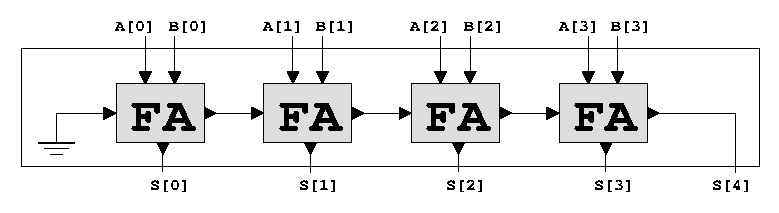
\includegraphics{figures/adder}
  }
\caption{Addition of integers coded in boolean, using \emph{full adders}\label{adder}}
\end{figure}

The following system is a \emph{full adder} function written in {\alfa}. 
\index{full adder}

\begin{verbatim}
      system FullAdder (A,B,Cin : boolean) 
               returns (X,Cout : boolean);
      let
        X = A xor B xor Cin;
        Cout = (A and B) or (A and Cin) or (B and Cin);
      tel;
\end{verbatim}



To build an adder system with this program, we need to be able to
express that we have a linear collection of instances of this system,
as shown in Fig.\ref{adder}. The shape of this linear collection may
be expressed as an {\alfa} domain, say \texttt{\{b|0<=b<W\}} where
\texttt{W} is a size parameter giving the number of bits.
\index{use statement}

The structure construct \textbf{use} in {\alfa} allows precisely that:
the following system describes in {\alfa} the adder given Fig.\ref{adder}: 
\index{adder}\index{binary addition}

\begin{verbatim}
     system Plus: {W|W>1} (A,B: {b| 0<=b<W} of boolean)         -- 1  
                  returns (S : {b| 0<=b<=W} of boolean);        -- 2  
     var                                                        -- 3  
       Cin, Cout, X : {b| 0<=b<W} of boolean;                   -- 4  
     let                                                        -- 5  
       use {b| 0<=b<W} FullAdder[] (A,B,Cin) returns(X, Cout);  -- 6  
       Cin[b] =                                                 -- 7  
         case                                                   -- 8  
           {| b=0} : 0[];                                       -- 9  
           {| b>0} : Cout[b-1];                                 -- 10 
         esac;                                                  -- 11 
       S[b] =                                                   -- 12 
         case                                                   -- 13 
           {| b<W} : X;                                         -- 14 
           {| b=W} : Cout[W-1];                                 -- 15 
         esac;                                                  -- 16 
     tel;                                                       -- 17 
\end{verbatim}


\index{use statement}
In this system, the line 6 reads as follows: ``Use a collection of
instances of the subsystem \texttt{FullAdder}. This collection has the
shape of the extension domain\index{extension domain} \verb!{b|0<=b<W}! 
and is thus indexed by index \texttt{b}. Let the inputs of
the \texttt{b}-th instance be the variables \texttt{A}, \texttt{B} and
\texttt{Cin} at point
\texttt{b}, and similarly let the outputs of this collection of
instances be the variables \texttt{X} and \texttt{Cout}.''
(The lines~7-11 describe the carry propagation, and lines~12-16
define the output of this binary adder.)

\index{dimension extension}
In other words, line~11 is a shortcut for the following equations,
which are those of the system \texttt{FullAdder} whith the dimension
of the variables extended from zero to one:

\begin{verbatim}
        X[b] = A[b] xor B[b] xor Cin[b];
        Cout[b] = (A[b] and B[b]) or (A[b] and Cin[b]) or (B[b] and Cin[b]);
\end{verbatim}





\section{Syntax of the \emph{use} construct}

\index{use syntax}
The \textbf{use}\ construct appears at the syntactic
level of an equation, since it is basically a shortcut for a set of
equations. Here is the general syntax of an equation/use:
{\tt
\begin{tabbing}
xxx\= xxx\= xxx\= xxx\= xxx\= xxx\= xxx\= xxx\= xxx\=  \kill
\textsl{Equation} ::\\
\>\> \textsl{Identifier} = \textsl{Expression} ;\\
\> \Alt\ \> use \Opt{ \textsl{ExtensionDomain}} \textsl{Identifier}\\
\>\>\>\>\>\> \Opt{[\textsl{ParamAssignment} ]} \\
\>\>\>\>\>\>( \textsl{ExpressionList} )\\
\>\>\> returns\>\>\> ( \textsl{IdentifierList} ) ;
\end{tabbing}
}
 

\index{parameter assignment}\index{assignment of the
parameters}\index{parameters}
In this syntax we see that there is an optional \emph{parameter
assignment} which is discussed in the following.
In the previous addition, the subsystem \texttt{FullAdder} has
no parameters, and the parameter assignment is therefore empty. 




\section{Binary multiplication in {\alfa}}

When performed by hand, a multiplication is basically a collection
of additions, as shown by Fig.\ref{intmul}. \index{binary multiplication}

\begin{figure}[!ht]
\begin{center}
    \includegraphics{figures/intmul}
  \caption{Product of two fixed point reals in binary representation\label{intmul} }
\end{center}
\end{figure}


The following program is the {\alfa}
incarnation of Fig.\ref{intmul}. Line~8 performs the binary product of
all the bits of the first operand by each bit of the second. Line~10
describes a linear collection of additions, indexed by \texttt{m}
which is the row index in Fig.\ref{intmul}. Lines~12-17 link the
result of one additions to the input of the following. 

\begin{verbatim}
    system Times: {W|W>2} (A,B: {b| 0<=b<W} of boolean)   -- 1  
                  returns (X  : {b| 0<=b<W} of boolean);  -- 2  
    var                                                   -- 3  
      P : {b,m| 0<=b,m<W } of boolean;                    -- 4  
      Si : {b,m| 0<=b<W; 0<m<W } of boolean;              -- 5  
      So : {b,m| 0<=b<=W; 0<m<W } of boolean;             -- 6  
    let                                                   -- 7  
      P[b,m] = A[b] and B[m];                             -- 8  
      use {m| 0<m<W} Plus[W] (Si,P) returns (So);         -- 9   
                                                          -- 10 
      Si[b,m] =                                           -- 12 
                                                          -- 11
        case                                              -- 13 
          {| m=1} : P[b,m-1];                             -- 14 
          {| m>1} : So[b+1,m-1];                          -- 15 
        esac;                                             -- 16 
      X[b] = So[b+1,W-1];                                 -- 17 
    tel;                                                  -- 18 
\end{verbatim}


Here the parameter assignment \texttt{W} just equates the bit size
parameter of the subsystem \texttt{Plus} and that of the
multiplication. In the general case, however, this parameter
assignment may be any affine function, which proves very
powerful. Figure~\ref{accumdraw} describes the problem of accumulating
binary numbers without overflow: the sum of two $N$-bits numbers may
be a $N+1$ bits number, therefore we need to use additions of
increasing sizes to avoid loss of bits. This is expressed in {\alfa} as:
\begin{verbatim}
         use {i| 1<=i<N} Plus[W+i-1] (A1,A2) returns (Acc);
\end{verbatim}
\index{parameter assignment}\index{assignment of the
parameters}\index{parameters}
\begin{figure}[!ht]
\centerline{
   \includegraphics{figures/Accum}
    }
\caption{Binary numbers accumulation. \label{accumdraw} }
\end{figure}

Another example where the natural structuring of an algorithm
makes use of a parameter assignment depending on the extension indices
is the Gaussian elimination given at the beginning of
chapter~\ref{static}. The reader is invited to try and understand this
program.

\index{extension domain}
Note that in all our examples, the extension domain is
monodimensional, but this is not a rule: in the general case the
extension domain may be any arbitrary {\alfa} domain. For example, in
an image processing application, a 2-dimensional extension domain may
be used to apply some function to all the points of an image.

\section{Manipulating structured programs}

A structured program is stored in {\mmalfa} as a {\mma} list of
systems called a \emph{library}. The default library is stored in the
global variable \verb!$library!.\index{$library}

A structured program may be written in one single file or several
distinct files.  In the latter case the \texttt{load[]} function
returns a library composed of all the systems contained in the file,
and stores this library in \verb!$library!. %$ 

If the program is stored in several files, it is the responsibility of
the user to build a proper library, i.e. a {\mma} list of all the
systems needed by the hierarchical structure of the program. For this
purpose, the user will typically use {\mma} list manipulating
functions such as \texttt{Join[], Append[]}...\index{structured
programs}

In addition, two functions, \texttt{putSystem[]} and
\texttt{getSystem[]}, may be used to extract a system from a library
and to put back a modified system in a library. Typically one of the
system is extracted from the library, modified by some program
transformation, and then put back in the library.\index{putSystem[]}\index{\getSystem[]}




\section{Program transformations associated with structures}

Most {\mmalfa} functions handle parameterized programs and \emph{use}
statements. There are, however, some major exceptions such as the
\texttt{writeC[]} translator. \index{writeC[]}In this case, {\mmalfa}
provides program transformations transforming a structured program
into a simpler equivalent one~:

\begin{itemize}

\item \texttt{assignParameterValue[]} \index{assignParameterValue[]}
gives a value to a size parameter, i.e. it refines a generic system
into a specialized one.

\item \texttt{inlineSubSystem[]} \index{inlineSubSystem[]} expands a
\emph{use} statement, replacing it with the equations of the
corresponding subsystem, properly modified to take the dimension
extension into account.\index{flattenning a structured program}

\item \texttt{inlineAll[]} \index{inlineAll[]} recursively flattens a
structured {\alfa} program.

\end{itemize}















% Analyze

\chapter{Static analysis of {\alfa} programs\label{static}\label{chapanalyze}}

\section{Introduction}


This chapter describes the use of the static analysis tool
\texttt{analyze[]}.\index{analyze[]}  
It is divided in two parts: the first part deals with the
static analysis of a single system, and the second describes the
analysis of a structured program consisting of several systems. Any
beginner in {\alfa} should read the first part, while the
second part is left to more experienced users.



\subsection{What is static analysis?\index{static analysis}}

It is impossible to ensure that an {\alfa} system computes the
expected result (to start with, the termination of such computation is
well known to be indecidable). However there are a few necessary
conditions for a system to be valid which may be verified
\emph{statically}, that is

\begin{itemize}

\item independently of any set of input values that may be fed to the
system, and
\item in a manner that is valid for any of these set of values.

\end{itemize}


\subsection{What does the static analyzer do?}

The {\alfa} static analyzer basically verifies the following rule:

\emph{For each point of the domain of a variable, there is
one and only one computation defining the value of the variable at
this point.}

The static analyzer checks that this rule is ensured and outputs error
messages giving the points where a variable is over- or under-defined.



\subsection{When should the static analyzer be used?}

This tool is very useful while writing and debugging {\alfa} code, and
should be invoked systematically. Besides, 

{\large
\begin{center}
\emph{{\alfa} program transformations are only guaranteed to work}

\emph{on programs that pass the static analysis without error messages.}

\end{center}
}

This is in particularly true of the {\alfa} to C translator \index{writeC}
\texttt{writeC[]}: the C code generated by this command is likely to
cause run-time errors if the initial {\alfa} program doesn't pass the
static analysis. Therefore the static analyzer should be called before any
simulation of the {\alfa} program.


\subsection{An example\index{gaussian elimination}}

We will use in this chapter the following two-system example program
which transforms a matrix into triangular form as first step of a
Gaussian elimination\footnote{This program is neither optimal nor
complete, it was written for the purpose of demonstrating the
\textsc{analyze[]} function. Writing a complete Gaussian elimination
is left as an exercise to the reader.}.

The first system takes a square matrix and zeroes all the elements
below the \texttt{K}-th diagonal of this matrix (one slice of
Fig.\ref{gauss-slices}):

\begin{verbatim}
 system ZeroColumn: {N,K| 1<=K<N} (A: {i,j| 1<=i,j<=N} of real)
                          returns (Ar: {i,j| 1<=i,j<=N} of real);
 let
   Ar[i,j] = case
             {| i<=K}      : A[i,j];
             {| i>K; j<=K} : 0[];
             {| i>K; j>K}  : A[i,j] - A[K,j]*A[i,K]/A[K,K];
             esac;
 tel; 
\end{verbatim} 

The second system uses N instances of the first to compute the
triangular matrix (see Fig.ref{gauss-slices}):

\begin{verbatim}
 system Gauss: {N | N>1} (A: {i,j | 1<=i,j<=N} of real)
                 returns (T: {i,j | 1<=i,j<=N} of real);
 var Ak : {i,j,k| 1<=i,j<=N; 1<=k<=N} of real;
     Ak1: {i,j,k| 1<=i,j<=N; 1<=k<N} of real;
 let
   use {k| 1<=k<N} ZeroColumn[N,k] (Ak) returns (Ak1);
   Ak[i,j,k] = case
               {| k=1} : A[i,j];
               {| k>1} : Ak1[i,j,k-1];
               esac;
   T[i,j] = Ak[i,j,N];
 tel;
\end{verbatim} 

\begin{figure}
\centerline{
	\includegraphics[width=8cm]{figures/gauss}
        }
\label{gauss-slices}
\caption{Triangularization in two systems}
\end{figure}



What kind of information does the static analyzer give? Suppose a typo
has replaced an \texttt{j} index with a \texttt{i} index, leading to
the following \texttt{ZeroColumn} program:

\begin{verbatim}
 system ZeroColumn: {N,K| 1<=K<N} (A: {i,j| 1<=i,j<=N} of real)
                          returns (Ar: {i,j| 1<=i,j<=N} of real);
 let
   Ar[i,j] = case
             {| i<=K}      : A[i,j];
             {| i>K; i<=K} : 0[];     -- The typo is hidden here
             {| i>K; j>K}  : A[i,j] - A[K,j]*A[i,K]/A[K,K];
             esac;
 tel;
\end{verbatim} 

This error can't be detected by a parser program -- this program is
syntactically correct. However, invoking the static analysis will
yield the following messages:\index{analyze[]}

\begin{verbatim}
In[5]:= analyze[];
 
WARNING: This expression has an empty domain :
{i,j | i=0; j=0; N=0; K=0; 1=0} : 0.(i,j->)
 
ERROR: Variable Ar not defined over the domain :
{i,j | K+1<=i<=N; 1<=j<=K}
 
*** Analysis failed ***
\end{verbatim}

A warning and an error tell us that there is an error in the equation
defining \texttt{Ar}. Several \emph{error domains} may help us pinpoint
precisely where the error is. The first warning message is enough
to spot that the error is in the \texttt{case} subexpression
containing the \texttt{0[]}. The \texttt{1=0} equation in the domain
indicates that this domain is empty.\index{empty domain}

As this example shows, it may take a certain amount of experience
to fully understand the error messages: the error domains
are not always in the most readable form. However the indications
given usually allow to spot the problem precisely: in our example the
combination of both previous messages points exactly to the cause of
the error.


The remainder of this paper describes the static analysis tool in more
details.



\section{Static analysis of an {\alfa} system}
\label{static-analysis}


\subsection{The domain of an expression\label{expr_check}}

\index{expression domain}\index{domain of an expression} In {\alfa}
every variable is declared with a polyhedral domain defining the set
where it is expected to contain a value.\index{declaration
domain}\index{domain of a variable}

When an expression is built using such variables, this expression
inherits the domain of these variables: for example if \texttt{A} and
\texttt{B} are two expressions defined over some square domain
\texttt{\{i,j|0<i,j<10\}}, then their
sum \texttt{A+B} is defined everywhere both \texttt{A} and \texttt{B}
are defined, that is on the same square domain.

Now if the domains of \texttt{A} and \texttt{B} are different, then
the sum is still defined everywhere both \texttt{A} and \texttt{B} are
defined, that is on the intersection of the domains of \texttt{A} and
\texttt{B}.

It is possible to carry these ideas further, and thus to define the
domain of any {\alfa} expression, knowing the domains of the
subexpressions (see the discussion of section~\ref{arrayform},
page~\pageref{arrayform}). The rules to apply, given below, are actually part of
the definition of the semantics\index{semantics of {\alfa}} of the
language. They rely only on operators preserving the set of {\alfa}
domains and thus may be computed automatically: this is what the
static analyzer does.


 \begin{center}
  \begin{tabular}{rc}
   {Constants} & \fbox{$Dom(c) = \mathbf{Z}^0$} \vspace{1ex}\\ 
   {Variables} & \fbox{$Dom(V) \textrm{ is declared in the header}$}\vspace{1ex}\\ 
   {Unary operators} & \fbox{$Dom(-e) = Dom(e)$}\vspace{1ex}\\ 
   {Binary operators} & \fbox{$Dom(e_1+e_2) = Dom(e_1) \cap Dom(e_2)$}\\
   & {\small The sum of two variables is defined where both variables are defined}\vspace{1ex}\\ 
   {Ternary operators} & \fbox{$Dom(\texttt{if}\ e_1\ \texttt{then}\ e_2\ \texttt{else}\ e_3) = 
            \bigcap_{i=1}^3 Dom(e_i)$}\\
   & {\small The \texttt{if}\ \texttt{then}\ \texttt{else}\ is considered as a ternary operator}\\
   & {\small and is defined where the condition and both alternatives are defined}\vspace{1ex}\\ 
   {Restriction} & \fbox{$Dom(D : e) = D\cap Dom(e)$}\\
   {\small $D$ is a domain} 
   & {\small This operator restricts an expression to D}
   \vspace{1ex}\\
   {Affine dependency} & \fbox{$Dom(e[f]) = f^{-1}(Dom(e))$}\\
   {\small $f$ is an affine function}
    & {\small The value of $e[f]$ at point \textbf{z} is the value of $e$}\\
   {\small of the indices of the LHS}
    & {\small at point $f(\mathbf{z})$, hence the domain of $e[f]$}
  \vspace{1ex}\\
   {\texttt{case} operator} 
   & \fbox{$Dom(\texttt{case} e_1;..;e_n;\texttt{esac}) = \bigcup_{i=1}^n Dom(e_i)$}\\
   & {\small The \texttt{case} operator allows the piecewise definition of an expression}\\
   & {\small by several subexpressions $e_i$ with disjoint domains.}
  \end{tabular}
 \end{center}

The function \texttt{expDomain[]} \index{expDomain[]} may be used to
compute the domain of any {\alfa} expression, following these rules.

Now during the computation of the domain of an expression, the
\texttt{case} operator \index{case} introduces the possibility of
having more than one subexpression define the value of the same point
of the domain.  Therefore the analysis tool has to check that the
intersections of the domains of the case subexpressions are empty. It
computes this intersection, and if it not empty it issues an error
message as in the following example:
\index{overlap of case statements}\index{analysis of the case}\index{case validity}

\textbf{Example:} in the equation defining \texttt{Ar}, if the
second line of the \texttt{case} was wrongly written:
\begin{verbatim}
      {| i>=K; j<=K}: 0[];
\end{verbatim}
The analysis tool will output the following message:
\begin{verbatim}
 ERROR: in case statement: ...,
        domains of subexpressions overlap on:
        {i,j | i=K; 1<=j<=K}
\end{verbatim}


There are other useful informations which the static analyzer
provides. For example it is useful to detect an empty expression
i.e. an expression with an empty domain: such an expression is 
in the best case pointless (in a case statement), and may be a source of
errors. \index{expression has an empty domain}\index{empty domain}
To avoid cascaded error messages, only the
deepest empty subexpression is reported to the user.

\textbf{Example:}
 Still in the same equation, a mistake in the first \texttt{case} subexpression:
\begin{verbatim}
      {| i<=0}     : A[i,j];
\end{verbatim}
will cause the following messages:
\begin{verbatim}
 WARNING: This expression has an empty domain: 
          {| i<=0} : A[i,j]
 ERROR:   Variable Ar not defined over the domain: 
          {i,j| 1<=i<=K; 1<=j<=N}
\end{verbatim}



\subsection{Equation analysis\label{equ_check}}

\index{equation analysis}\index{analysis of an equation} Now we
describe how the static analyzer works: it considers each equation
$V[i,j\ldots] = e$, where $e$ is an {\alfa} expression.  To ensure
that there is at least one computation defining the value of $V$ for
each point $(i,j,\ldots)$ of its domain, the analysis tool computes
$D' = Dom({V}) \setminus Dom({e})$, where $\setminus$ denotes the set
difference, $Dom(V)$ is the domain of the variable $V$ (declared in
the header of the system), and $Dom(e)$ is the domain of the
expression as defined above.\index{declaration domain}\index{domain of
a variable}
 
If $D'$ is non empty, an error is issued, stating that $V$ is not
defined over $D'$. This error domain will be useful to the user to
spot the problem. \index{variable not defined}

\textbf{Example:} In the equation of the system \texttt{ZeroColumn} 
 defining \texttt{Ar}, 
suppose the first line of the \texttt{case} statement was mistyped:
\begin{verbatim}
      {| i<K}     : A[i,j];    -- instead of {| i<=K} ...
\end{verbatim} 
(notice the \verb~<K~ instead of \verb~<=K~). The analysis tool will output
 the following message:
\begin{verbatim}
 ERROR: Variable Ar not defined over the domain:
        {i,j| i=K; 1<=j<=N}
\end{verbatim} 




\subsection{Parameter related analysis\label{param-check}}

\index{parameter analysis}\index{analysis of a parameterized system}
If the system considered is parameterized, the static analysis process
may be usefully refined by taking the parameters into
account. Consider again the \texttt{Gauss} system:

\begin{verbatim}
 system Gauss: {N | N>1} (A: {i,j | 1<=i,j<=N} of real)
                 returns (T: {i,j | 1<=i,j<=N} of real);
 var Ak : {i,j,k| 1<=i,j<=N; 1<=k<=N} of real;
     Ak1: {i,j,k| 1<=i,j<=N; 1<=k<N} of real;
 let
   use {k| 1<=k<N} ZeroColumn[N,k] (Ak) returns (Ak1);
   Ak[i,j,k] = case
               {| k=1} : A[i,j];
               {| k>1} : Ak1[i,j,k-1];
               esac;
   T[i,j] = Ak[i,j,N];
 tel;
\end{verbatim} 


Suppose there was no restriction on the parameter \texttt{N} of the
system \texttt{Gauss}. Its header would be: \mbox{\verb~ system Gauss:
\{N |\} ~}.  Now obviously for negative values of \texttt{N}, all the
variables of this system have an empty domain, \index{expression has
an empty domain}\index{empty domain} which should be pointed to the
user as a possible source of errors.  The static analyzer performs
such parameter-related checks.

\textbf{Example:}
 We may restrict the parameter \texttt{N} of the system \texttt{Gauss} to
 be positive:
\begin{verbatim}
 system Gauss: {N | N>0}  
\end{verbatim}
One may check that the system is still valid, even for \texttt{N=0}.
 However the analysis will issue the following message:
\begin{verbatim}
 WARNING: for parameters {N| N=1}, the expression Ak1 has an empty domain
\end{verbatim}


It is good programming practice to ensure that the system is valid for
all the values of its parameter domain. It becomes mandatory if the
program is composed of several systems, as shown in the following
section.




\section{Analysis of structured programs}
\index{analysis of structured programs}

\subsection{Analysis of \texttt{use}\ statements\label{useanalysis}}
\index{analysis of the use}\index{use statement analysis}\index{validity of the use}

The analysis of a \texttt{use} statement is deduced from its
\index{substitution semantics}\index{semantics of the use}
\emph{substitution semantics}: in short, a program containing a
\texttt{use}\ statement is (by definition of the use) equivalent to
one where this statement has been replaced with the body of the
subsystem (properly modified to take into account the extra dimensions
and the affine parameter assignment) and additional equations to
perform the I/O passing: input equations relate the actual inputs and
the formal ones~:
\begin{verbatim}
      SubSystemInputVariable = ActualInputExpression ;
\end{verbatim} 
and output equations relate the actual outputs and the formal ones~:
\begin{verbatim}
        ActualOutputVariable = SubSystemOutputVariable ;
\end{verbatim} 


\paragraph{Global checks}
The first validity conditions are that the subsystem has been declared
somewhere in the program, that the correct number of actual
inputs/outputs are given, and that their respective dimensions match
the formal ones.  The tool also checks, using the same techniques as
previously, that the extension domain is non-empty for all the values
of the parameters.

\index{parameter assignment}\index{assignment of the
parameters}\index{parameters}\index{validity of the parameter
assignment} 
Then we consider the values given to the parameters of
the subsystem by the caller. The parameters of the subsystem are
an affine function of the caller parameter and,
possibly, the extension indices.  The analyzer checks that, for all
the possible values of the caller parameters, and for all the points
in the extension domain, the values assigned to the subsystem
parameters fall within the range permitted, i.e. within the parameter
domain of the subsystem.  Otherwise an error message is issued,
showing a domain which is the set of points where parameters are given
but not expected.


\textbf{Example:}
In the \texttt{Gauss} system, the following \texttt{use}\ statement:
\begin{verbatim}
    use {k| 0<=k<=N} ZeroColumn[N,k] (Ak) returns (Ak1);
\end{verbatim}
will cause the following message:
\begin{verbatim}
 ERROR : in statement ``use ... ZeroColumn...'',
         parameter values in {N,K| K=0, N>=1} not allowed.
\end{verbatim}
 
Obviously, the more restricted the parameter domain of the subsystem,
the more acurate the checks performed here.


\paragraph{Input/Output checks}

\index{subsystem input/output}
The substitution semantics implies that the verifications to be
performed on the I/Os of a subsystem \texttt{use}\ may be deduced from
those of the equations described in \ref{equ_check}. Error messages
are given accordingly.



\subsection{Global analysis of a library of systems}

\index{analysis of a structured program}
The validity of a \texttt{use}\ statement is then implied by the
validity of the subsystem on its parameter domain, the condition that
all the parameter values assigned by a \texttt{use} are allowed, and
the validity of the virtual I/O passing equations.

We may thus describe the general down-top verification method for a
complete program. Such a program is an acyclic graph of {\alfa}
systems using each other (system \texttt{use} can not be mutually
recursive). Systems without a \texttt{use}\ statement in their
equations are called {\em leaves}. A system using a subsystem is
called a {\em parent} of this subsystem.
\begin{itemize}
\item First, the leaves are analyzed, and their parameter domain is
restricted as much as possible. No warning message should remain.  For
example, for the system \texttt{ZeroColumn}, we have to restrict
\texttt{K} and \texttt{N} at least to the domain given in the
correct version of this sytem (it is possible to constraint the
parameters more than what the analysis suggests. For example we could
put a bound on \texttt{N} depending on the application aimed at).

\item Then the parents of the leaves are analyzed. If they are written
to use a leaf with illegal values of its parameters, the tool
will spot it and the programmer will be invited either to correct the
error, or to restrict more the caller parameters. Meanwhile, the other
equations of the caller are also analyzed, with the same effect.

\item This process is repeated on the parents of the parents, and so
on until the whole program passes the static analysis.
\end{itemize}

Note that one of the options to \texttt{analyze[]} decides whether the
analysis is performed recursively on all the subsystems of the system
currently being analyzed, or only to this system.




% Code generation

\chapter{Code generation and simulation of {\alfa} programs}
\label{chapcodegen}
In this chapter, we explain how to generate C code from an
{\alfa} program. As seen in Chapter~\ref{chapfunctional}, 
{\alfa} programs are functional, and therefore, do not convey any
execution ordering. However, the validation of {\alfa} programs, 
or even, the generation of code for a general-purpose or
dedicated processor, requires the possibility to simulate the 
evaluation of {\alfa} expressions. 

This can be done using the {\tt writeC} {\mmalfa} command, as seen here.

\section*{An example}
Consider the following {\alfa} program:
\begin{figure}[htbp]
%\htmlimage{scale=\myscale}
\verbatiminput{alpha_progs/adder-WriteC.alpha}
\caption{A very simple example\label{adderwritec}
}
\end{figure}
To simulate this program, we first load this program, 
then generate a C program in file ``adder.c'', using 
\begin{verbatim}
load["adder-WriteC.alpha"];  (* load file *)
writeC["adder.c"];
\end{verbatim}
Then we can compile this program: 
\begin{verbatim}
cc -o adder adder.c
\end{verbatim}
The execution of this program is shown here:
\begin{verbatim}
adder
Input x =2
x = 2
Input y =3
y = 3
z = 5
\end{verbatim}
The C code prompts for the value of the input variables {\tt x} and
{\tt y}.
\section{Program with parameters}
Programs with parameters cannot be simulated without giving 
a value to the parameters. This is obtained through an option of
{\tt writeC}. 
\begin{figure}[htbp]
%\htmlimage{scale=\myscale}
\verbatiminput{alpha_progs/adder-WriteC1.alpha}
\caption{A very simple example\label{adderwritec1}
}
\end{figure}
\begin{verbatim}
load["adder-WriteC1.alpha"];  (* load program *)
writeC["adder1.c","-p 3"];
cc -o adder1 adder1.c
adder1Input x[1] =2
x[1]= 2
Input x[2] =3
x[2]= 3
Input x[3] =4
x[3]= 4
Input y[1] =-2
y[1]= -2
Input y[2] =-3
y[2]= -3
Input y[3] =-4
y[3]= -4
z[1]= 0
z[2]= 0
z[3]= 0
\end{verbatim}
\subsection{Additional examples}
\begin{verbatim}
SetDirectory["/home/frodon/d01/api/quinton/alpha/sobel"];
load["sobel.a"];ashow[];
analyze[];
writeC["-p 5 35 3"];
schedule[{objFunction -> 1,addConstraints -> {"Tpixel[i,N,M,p]=i"},duration -> 2}]
\end{verbatim}



% Scheduling

\newcommand{\aalpha}{{\alfa}}
\newcommand{\lp}{{\sc lp}}
\chapter{\index{Scheduling}Scheduling {\alfa} programs}
\label{chapscheduling}

{\sc Version of \today}

This chapter explains how to use the scheduler for finding valid
execution order of computations of {\alfa} programs.
 
\section{Introduction}
An {\aalpha} program does not convey any sequential ordering: an
execution order is semantically valid provided it respects the data
dependencies of the program.  Consider for instance the program of
figure~\ref{figSched1} which represents the computation of the product
of a $M\times N$ matrix \texttt{a} by a $M$ vector \texttt{b}. To execute
such a program on a sequential machine, we must chose a
computation
order which respects data dependencies. Such an
order is shown in figure~\ref{figSched2}-(a). Another possible
order would be the demand-driven execution scheme used in the
simulation, as shown in chapter~\ref{chapcodegen}\,: to evaluate a
variable, evaluate recursively the expressions that this variable
depends on.  Parallel executions are also possible. The program of
figure~\ref{figSched2}-(b) shows a possible parallel order for
computing the matrix-vector multiplication.  

\begin{figure}[htbp]
%\htmlimage{scale=\myscale}
\verbatiminput{alpha_progs/MatVect.alpha}
\caption{{\aalpha} program for the matrix-vector product, 
no execution order is specified.}
\label{figSched1}
\end{figure}

\begin{figure}[htbp]
%\htmlimage{scale=\myscale}
\begin{minipage}{8cm}
\begin{verbatim}
For i=1 to N
   C[i,0]=0
EndFor
For i=1 to N
   For j=1 to M
       C[i,j]=C[i,j-1]+
                a[i,j] * b[j]
   EndFor
EndFor
For i=1 to N
   c[i]=C[i,M]
EndFor

           (a) 
\end{verbatim}
\end{minipage}
\begin{minipage}{8cm}
\begin{verbatim}
ForAll i=1 to N
   C[i,0]=0
EndFor
For j=1 to M
   ForAll i=1 to N
       C[i,j]=C[i,j-1]+
                 a[i,j] * b[j]
   EndForAll
EndFor
ForAll i=1 to N
   c[i]=C[i,M]
EndForAll

           (b)
\end{verbatim}
\end{minipage}
\caption{
Two possible order of execution for the program of figure~\ref{figSched1}. The 
left one is parallel. (\texttt{ForAll} represents a parallel loop).}
\label{figSched2}
\end{figure}

The basic goal of the scheduler is to find out valid execution orders, 
called {\em schedules} in what follows. 
A secondary goal is to find out {\em good} schedules. 
However, there is no best schedule: the quality of
a schedule depends on a particular criterion. 

In our model, the time is considered as a discrete single clock and we
look for parallel ordering of the computations.  The theoretical basis
for the scheduling process is inherited from the research on systolic
array and automatic parallelization. The scheduler implements two
different procedures: one, called the Farkas method, is defined
in~\cite{Feautrier92aa}; the other one, called the vertex method, is
presented in~\cite{citationdespaa}.

The scheduler of \alfa{} is an analysis tool: it does not modify the
current program in \texttt{\$result}.  The result is the description of a
possible parallel schedule. For instance, for the program of
figure~\ref{figSched1}, if we assume that the inputs are available at
time 0 and that each assignement takes 1 clock tick, we
will obtain the information that, for all \texttt{i}, value {\tt
C[i,j]} can be computed at step \texttt{j}.  Thus, for all \texttt{i}, the
values \texttt{c[i]} can be computed at step \texttt{M+1}. This schedule
can be summarized by:
\begin{equation}
\label{Schedeqn1}
\begin{array}{l} T_a[i,j] = 0 \\ T_b[i] = 0 \\ 
T_C[i,j] = j \\ T_c[i] = M+1 \end{array} 
\end{equation}
This particular schedule corresponds exactly
to the parallel execution order of the program of figure~\ref{figSched2}-(b).

In the present chapter, we are interested in {\em affine by variable}
schedules, i.e schedules in which, for each variable, the execution
date is an affine function of the indices (and possibly of the
structural parameters). The idea of the scheduling process is to
gather all the constraints that the schedule must verify in a linear
programming problem ({\sc lp}) and to solve this \lp{} using a {\sc lp}-solver.

\section{Basic Farkas scheduler}

The scheduling process is quite complex, since many parameters
can influence the result. In this section, 
we present the basics of the scheduler.

\subsection{How to use the \texttt{schedule} function}

The function to be called in order to schedule a program is {\tt
schedule}. Its effects is to find out a schedule for the {\aalpha} program
contained in \texttt{\$result}, and to put the schedule in the
global \mma{} variable \texttt{\$schedule}. Options allow one to modify
parameters, hence the possible forms of a call to the function {\tt
schedule} listed here: 
\begin{itemize}
\item \texttt{schedule[]}\\ finds an affine-by-variable schedule for {\tt
\$result} and assigns it to
\texttt{\$schedule} (this schedule attempts to  minimize
 the global execution time).
\item \texttt{schedule[sys]}\\ 
finds an affine-by-variable schedule for the {\aalpha} system \texttt{sys}
 and assigns it to
\texttt{\$schedule}
\item {\tt
schedule[option\_1->value\_1,\ldots,option\_n->value\_n]}\\
finds a schedule for \texttt{\$result} which respects the chosen options and
assigns it to \texttt{\$schedule}
\item {\tt
schedule[sys,option\_1->value\_1,\ldots,option\_n->value\_n]}\\
finds a schedule for the {\aalpha} system \texttt{sys} which
 respects the chosen options and
assigns it to \texttt{\$schedule}
\end{itemize}

For example, calling the scheduler on the matrix-vector multiplication
of figure~\ref{figSched1} prints out the following informations:
\begin{verbatim}
In[30]:= schedule[];
Dependence analysis...
Duration : 1 for each equation 
Building LP...
LP: 82 Constraints
Writing file for PIP....
Solving the LP...
Version C.3 MultiPrecision (mpip, rev. 1.3.0)
cross : 407646, alloc : 1
Max cross-product result: 4 (1 digits, base 10)
Max numerator term: 8 (2 digits, base 10)
Max denominator: 2 (1 digits, base 10)
n 1 u 130''' s 11'''
T_a{i, j, N, M} = 0
T_b{i, N, M} = 0
T_c{i, N, M} = 1 + M
T_C{i, j, N, M} = j

Out[30]= scheduleResult[1, {{a, {i, j, N, M}, sched[{0, 0, 0, 0}, 0]}, 
   {b, {i, N, M}, sched[{0, 0, 0}, 0]}, {c, {i, N, M}, sched[{0, 0, 1}, 1]}, 
   {C, {i, j, N, M}, sched[{0, 1, 0, 0}, 0]}}]
\end{verbatim}
 
The first lines indicate which computations are performed.  The Farkas
scheduler first built a \lp{}, then writes this \lp{} in a file,
then calls a \lp{}-solver. Writing this file takes some time, thus
informations are displayed for the user not to become anxious.

The lines starting by \texttt{Version} are output by the \lp{}-solver
\pip{}. The result of calling Pip is then shown. Here, for
instance the schedule says that \texttt{B[i,j,k]} is computed at time
\texttt{i}. The result (after \texttt{Out[30]}) is the corresponding
\mma{} expression representing \texttt{\$schedule}.

For such a little program, only a few seconds are necessary to find
out a schedule. But it may take quite a long time for larger {\aalpha}
programs.

\subsection{Format of the output of \texttt{schedule}}

The output of the \texttt{schedule} function has a special form. 
It is enclosed in a structure whose head is
\texttt{Alpha`ScheduleResult}. The first argument of this
structure is the type of 
the schedule (integer, coded as the option scheduleType, 
see section~\ref{schedType}) and its 
second argument is the schedule itself. 
The syntax of this structure is:\\
\texttt{
<schedResult> ::= Alpha`scheduleResult[scheduleType\_Integer,\{sched...\}]\\
$\begin{array}{l} \mbox{ <sched>} ::= \\ ~\\  ~ \end{array}\begin{array}{l} \mbox{\{ nameVar\_String,}\\
          \mbox{ indices\_List,}\\
           \mbox{ Alpha`sched[tauVector\_List,constCoef\_Integer] \}}
\end{array}$
}\\
The effect of the \texttt{schedule} function is to assign this form 
to te global variable \texttt{\$schedule}.

Another example is given in section~\ref{ExampleSched}. 
A schedule can be displayed using the \texttt{show} command:
\begin{verbatim}
In[31]:=show[$schedule]

T_a{i, j, N, M} = 0
T_b{i, N, M} = 0
T_c{i, N, M} = 1 + M
T_C{i, j, N, M} = j

Out[31]:=
\end{verbatim}

\subsection{Using the result of the scheduler}

We may use the result of the scheduler as an information on the program, 
but we can also tranform the {\aalpha} program such that this information
become explicit in the program.  For instance, on the matrix-vector example, 
if we perform the \index{change of basis}change of basis
\texttt{(i,j -> j,i)} on variable \texttt{C}
and if we rename (for instance) 
the first index \texttt{t} and the second one \texttt{j},
we obtain the program of figure~\ref{figSched3}.

\begin{figure}[htbp]
%\htmlimage{scale=\myscale}
\verbatiminput{alpha_progs/MatVectSched.alpha}
\caption{Scheduled version of  program of figure~\ref{figSched1}}
\label{figSched3}
\end{figure}

This program is functionnaly equivalent to the one of figure~\ref{figSched1}
but it shows exactly at which clock tick each  value of the local variable
\texttt{C} is computed: \texttt{C[t,i]} is computed at step \texttt{t}. We call
a program which has this property a \index{scheduled program} {\em
scheduled} {\aalpha} program.  Of course, in a scheduled {\aalpha}
program, the first index of the local variables defines a partial
order which is compatible with data dependencies.

The scheduled program of figure~\ref{figSched3} has been obtained by
evaluating the expression
\index{applySchedule}\texttt{applySchedule[]}.  This command applies a
change of basis to each local variable of the program contained in
\texttt{\$result} in such a way that the first index in the new basis
represent the time. The change of basis is not performed on the inputs
and outputs, as otherwise the new program would not be equivalent to the
previous one. Another example of the use of \texttt{applySchedule[]}
is shown in section~\ref{ExampleSched}.

\section{Advanced scheduling}
In this section we introduce some of the parameters of the 
\texttt{schedule} command which allow more precise results to be
obtained.  A detailed description of this function can be found in
the documentation 
file \texttt{\$MMALPHA/doc/user/Scheduler\_user\_manual.ps}.

\subsection{Options of schedule}
The \texttt{schedule} function has many options. These options
have default values indicated hereafter. To change these
values, put one of the corresponding replacement
rules as a parameter to the
\texttt{schedule} function (see the example in section~\ref{ExampleSched}).

\paragraph{Option \texttt{scheduleType}}
\label{schedType}
This option gives the type of schedule.
Its possible values are:
\begin{itemize}
\item \texttt{scheduleType -> affineByVar} (default) 
affine by variable scheduling;
\item \texttt{scheduleType -> sameLinearPart} affine by variable scheduling with constant linear part;
\item \texttt{scheduleType -> ?}  affine by variable scheduling with constant linear part except for the parameters.
\end{itemize}

\paragraph{objFunction }
This option gives the objective function chosen. Its type is integer,
the possible values are:
\begin{itemize}
\item \texttt{objFunction -> 0 } (default) the total latency is minimized. 
\item \texttt{objFunction -> 1 } no objective function (the
coefficients of the scheduling vectors are minimized in a
lexicographic order).

It is mandatory not to minimize the total execution time when this 
time is not bounded (otherwise, the schedule will fail).
\end{itemize}

\paragraph{ratOrInt}
The resolution of the linear programming problem generated is done 
by the software {\sc mp}Pip which is an infinite precision version
 of the sofware {\sc pip}~\cite{Feautrier88a}. The resolution can be done with
integer programming or rational linear programming.
  This option indicates whether the resolution of the {\sc lp} by {\sc mp}Pip
 is
 done in integer mode (resulting scheduling vectors with integral
 coefficients) or in rationnal mode (resulting scheduling vectors may contains
 rationnal coefficients).  Its type is integer, the possible values
 are:
\begin{itemize}
\item \texttt{ratOrInt -> 0 } : rationnal solution.
\item \texttt{ratOrInt ->  1 } : (default) integer solution.
\end{itemize}

\paragraph{addConstraints}
This option allows to add some constraints to the {\sc lp} generated.
This option is very usefull to guide the scheduling process.
 Its type is a list of string, each string representing a constraint. The
 constraints authorized are affine constraints on scheduling
vectors.
There are two types of  constraint added, one can force a scheduling
vector value or simply set linear constraints on its components. 
\begin{itemize}
\item forcing a  variable $A$ to be schedule at time i+2j+2 can be done 
with the constraints: \texttt{"TA[i,j]=i+2j+2" }. 
\item for more precise constraint,  one can directly access to each components 
of the schedule functions of each variable. For instance \texttt{TAD2}
 will represent the variable coefficient of the second indice
 in the schedule of variable \texttt{A} (and \texttt{CA} will represent 
the constant part in the schedule of variable \texttt{A}).
 With these names, one can set linear constraints 
on these coefficients using operators \texttt{==} or \texttt{>=}. For instance,
\texttt{\{"TAD1 == 1","TAD2 == 2", "CA >= 2" \} } is the same constraint
as above except thar the constant is allowed to be greater than two.
\end{itemize}  
Example of use:\\
\texttt{schedule[addConstraints->\{"TA[i,j,N]=i+2j-2",
"TBD2==2","TBD1+2TCD3>=1"\}]}



\paragraph{duration} indicates how to count the duration of each computation. The possible value for the duration option are: 
\begin{itemize}
\item \texttt{duration -> \{\} }: (default) each equation takes 1 step
	 (whatever complex the computation is).
\item \texttt{duration -> \{Integer...\} }: 

The duration of each equation is given by the user. The list must
contain as many integer as there are variables (do not forget the
input variables). For instance on the program of figure~\ref{figSched1}, the
command \texttt{schedule[]} is equivalent to the command:
\texttt{schedule[duration->\{1,1,1,1\}]}.
\end{itemize}


\section{Another example}
\label{ExampleSched} 
Consider the program of figure~\ref{figSched4}, which represent a
uniform program for the \index{multiplication of matrices}
multiplication of matrices. in this section, we give the result of the
schedule with different options.
\begin{figure}[htbp]
%\htmlimage{scale=\myscale}
\verbatiminput{alpha_progs/MMunif.alpha}
\caption{Uniform matrix matrix product}
\label{figSched4}
\end{figure}

\paragraph{Default use}
If you type the following command (after having loaded the program of figure~\ref{figSched4}):\\
\texttt{schedule[]}\\
the result should be: 
\begin{verbatim}
T_a{i, j, N} = 0
T_b{i, j, N} = 0
T_c{i, j, N} = 1 + 2 N
T_B{i, j, k, N} = i
T_A{i, j, k, N} = j
T_C{i, j, k, N} = k + N

Out[14]= scheduleResult[1, {{a, {i, j, N}, sched[{0, 0, 0}, 0]}, 
   {b, {i, j, N}, sched[{0, 0, 0}, 0]}, {c, {i, j, N}, sched[{0, 0, 2}, 1]}, 
   {B, {i, j, k, N}, sched[{1, 0, 0, 0}, 0]}, 
   {A, {i, j, k, N}, sched[{0, 1, 0, 0}, 0]}, 
   {C, {i, j, k, N}, sched[{0, 0, 1, 1}, 0]}}]
\end{verbatim}
The result (after \texttt{Out[14]}) is the
Mathematica structure assigned to \texttt{\$schedule}.

\paragraph{Adding a constraint}
Suppose that the inputs \texttt{a[i,j]} and \texttt{b[i,j]} arrive
respectively at time \texttt{i+j} and \texttt{i+j+3}. Moreover, we
want a schedule of unique linear part (because this allow a locally
connected array to be obtained from a uniform program).  We have to
add the two constraints: \texttt{"Ta[i,j]=i+j"} and
\texttt{"Tb[i,j]=i+j+3"}. Also, we need to set the option scheduleType
to 2, hence the command is:
\begin{verbatim}
In[15]:= schedule[addConstraints->{"Ta[i,j]=i+j","Tb[i,j]=i+j+3"},
                   scheduleType->2]
\end{verbatim}
The result is 
\begin{verbatim}
T_a{i, j, N} = i + j
T_b{i, j, N} = 3 + i + j
T_c{i, j, N} = 5 + i + j + N
T_B{i, j, k, N} = 3 + i + j + k
T_A{i, j, k, N} = i + j + k
T_C{i, j, k, N} = 4 + i + j + k
\end{verbatim}

Note that the unique linear part option is applied on local variables
only (indeed, it cannot be enforced on inputs and outputs which do not have
the same number of indices.) After scheduling, one can obtain a
scheduled program by typing the command: \texttt{applySchedule[]}. The
result is the program of figure~\ref{figSched5}.

Warning: the \texttt{applySchedule} function finds the change of basis 
by unimodular completion of the scheduling vector. The unimodular 
completion is not always possible (for instance, if the scheduling 
vector is null), in that case, applySchedule will perform 
a generalized change of basis and add a new dimension to the domain of 
the corresponding variable. A warning is printed out during this operation.

\begin{figure}[htbp]
%\htmlimage{scale=\myscale}
\verbatiminput{alpha_progs/MMunifSched.alpha}
\caption{Scheduled  matrix matrix product}
\label{figSched5}
\end{figure}

\subsection{What if no schedule can be found?}
Due to the restriction to linear schedule, there may 
happen that the schedule function only answers: 
\texttt{No schedule was found, sorry...}
There maybe several reasons for that:
\begin{itemize}
\item The program is not semantically correct, try \texttt{analyze[]}.
\item There exists a schedule but the time is not bounded. 
In this case try with the option \texttt{objFunction} set to 1.
\item No affine one dimensional schedule exists. You can try to find
a multidimensional schedule with the \texttt{multiSched}.
\item No schedule exists (there is no way of solving this problem).
\end{itemize}

\section{To come soon}
\begin{itemize}
\item Multi-dimensional schedule.
\item Structured scheduling.
\item Data-flow scheduling. 
\end{itemize}






% Alpha0 

\chapter{The Alpha0 format}
\label{chapalfha0}

{\sc Version of \today}

In this chapter, we describe the {\Alpha0} format which is basically a non-structured version of the {\AlpHard} language. We also 
 describe the methodology to go from an {\Alpha} program to an {\Alpha0} program and then how to translate it into {\AlpHard}. 

\subsection{Definition of {\AlphaZ}}
{\AlphaZ} was introduced by C. Dezan in her Phd thesis
(\cite{dezan}). It was conceived as the lowest level of {\Alpha} or
equivalently as a subset of {\Alpha} which can describe circuits at the 
register transfer level. the main weakness of this subset came from the fact
that {\Alpha} programs were not structured.  Since, the structuring of
{\Alpha} was provided by F. Dupont~\cite{DupontQuRi95} and the
structured version of {\AlphaZ} was studied by P. Le
Mo\"enner~\cite{Patricia96}.  {\AlpHard} (described in
chapter~\ref{chapalphard}) is now intended to be this subset of
{\Alpha} with structural interpretation, from which we can translate
{\Alpha} into {\vhdl} or other {\sc rtl} description
languages. However, during the transformation path from {\Alpha} to
{\AlpHard}, the automatic structuring is a complicated process, hence
it appeared that the {\AlphaZ} format is still necessary as an
intermediate format with all the register transfer level informations
but in an unstructured form. We describe hereafter, the second version
 the {\AlphaZ} format (Alpha0v2) which is slightly different from the version described in~\cite{dezan}


% As a platform to {\AlpHard}, we need to remove the second point of
% the previous definition, namely the fact that all temporal domains are
% of the form $\{t~|~ t>=\}$. The other basic principles remains the same
% with slight differences. spatial cases contain no dependencies,
% connections are represented using a simple space dependency (no
% case). Temporal cases are always nested in a spatial case.
% Control initialization  equations are called {\em control} equation,
% the {\em Mirror} equations are the equations affecting  input, output 
% and control signal to local variables (hence, control signal 
% become data signals). All these descriptions are summarized by the following 
% definition:

An {\Alpha} program is in {\AlphaZ} form if it contains no {\tt use} statement
and if it meets the following conditions:

\begin{enumerate}
\item there exits, for all declared domains (except for the domains of 
inputs and outputs variables) an interpretation function for the indices
(see~\cite{dezan} for precise definition of {\em interpretation function}).
 Basically, each index is either 
a temporal index (indicating living dates of the signal) or a spatial index
(indicating in which processor the signal lives).


\item The equations of the system define the output and local
 variables.  Each operator involved in the equations has a structural
 interpretation. these equations are of four types: data equations,
 connection equations, control equations and mirror equations.
\begin{itemize} 
\item data equations define the different signals of the program
which are necessarily local variables.
They are composed of the following operators:  
\begin{itemize} 
  \item pointwise operators represent the corresponding combinatorial 
operators. 
  \item restriction are used to restrict the spatial interpretation of 
indices.
\item  dependencies are temporal dependencies representing registers 
or identity dependencies representing connections between two signal inside one cell.
\item case are spatial case allowing to gather several signals.
\item the {\tt if} operator (with nested {\tt case} in each branches)
is interpreted as a multiplexer.
\end{itemize}
\item connection equations are limited to the following form: a single
spatial dependency between two signals ({\tt A=B.(t,p->t,p-1)} for
instance).
\item control equations allow initialize control signals. they define signals
which are only temporal (no spatial indices).
\item Mirror equations: equation between input variables of the system and 
local variable of the system (only for interface). equation limited to an 
affine function applied to a variable ({\tt A[t,p]=a[f(t,p)]} for input mirror
equation and {\tt b[i,j]=B[f(i,j)]} for output mirror equations)..
\end{itemize}
\end{enumerate}

Examples of {\AlphaZ} programs are present in the directory 
{\tt \$MMALPHA/examples/Alpha0}, a small example is presented hereafter
 (figure~\ref{fig04}).

\section{From {\Alpha} to {\AlphaZ}}
The first attempt to go from High level specification in {\Alpha}
to {\sc rtl} specification in {\Alpha0} has been done be Sie and 
Wilde~\cite{SieWilde94}. This methodology has been 
extended and we discribe it briefly here, more informations
can be obtained by executing the Notebooks demos: {\tt Fir} and {Matvect}.

Consider the very simple program of figure~\ref{fig01}

{\small
\begin{figure}[h]
\begin{verbatim}
system NtimeNot :{N | 2<=N}
                (a : {i | 1<=i<=N} of boolean)
       returns  (b : {i | 1<=i<=N} of boolean);
var
  Acc : {i,j | 1<=i<=N; 1<=j<=N} of boolean;
let
  Acc[i,j] = 
      case
        {| j=1} : a[i];
        {| 2<=j} : not Acc[i,j-1];
      esac;
  b[i] = Acc[i,N];
tel;
\end{verbatim}
\caption{An {\Alpha} program computing {\tt N} times {\tt Not} 
on an array {\tt a}}
\label{fig01}
\end{figure}
}

Translating the program in {\AlphaZ} consists in the following steps: 
\begin{enumerate}
 \item {\bf Uniformize the program}. Here the program is already
uniform, in general this procedure may be complicated {\mmalpha}
provides tools for the automatic or designer-guided uniformization
(see the documentation on the chapter~\ref{chapuniformize}).
\item {\bf Schedule the program}. It consists in finding an execution
date (and a place also) for each computation. Usually, once
uniformized, the program should be scheduled with a unique linear part
(see the chapter~\ref{chapscheduling} for detail on scheduling). The
function {\tt applySchedule} choose an allocation function. In our example, 
you can execute  the following commands:
\begin{verbatim}
schedule[]
applySchedule[]
renameIndices[{"t","p"}]
\end{verbatim}
We obtain a linear array of processors,
the resulting program is shown in figure~\ref{fig02}
{\small
\begin{figure}[h]
\begin{center}
\begin{verbatim}
system NtimeNot :{N | 2<=N}
                (a : {i | 1<=i<=N} of boolean)
       returns  (b : {i | 1<=i<=N} of boolean);
var
  Acc : {t,p | 1<=t<=N; 1<=p<=N} of boolean;
let
  Acc[t,p] = 
      case
        {| t=1} : a[p];
        {| 2<=t} : not Acc[t-1,p];
      esac;
  b[i] = Acc[N,i];
tel;
\end{verbatim}
\caption{Program of figure~\ref{fig01} after applying schedule}
\label{fig02}
\end{center}
\end{figure}
}

\item {\bf Pipeline Inputs and Output}. You can see in figure~\ref{fig02}
that the  {\tt a} is input in every processors. If we want only the first processor to input data from the host, we could have pipelined the input with the following command:\\
\verb/pipeIO["Acc","a.(t,p->p)","aIn.(t,p->t+1,p+1)","{t,p| p>=1}"]/. We can do the same treatment for the output. Here we chose not to pipeline the I/O for sake of simplicity.

\item {\bf Go Down to Alpha0}. When the previous steps have been correctly 
executed, this step should be automatic with {\tt toAlpha0v2[]} command. In 
Our case, if we apply this function to the program of figure~\ref{fig02},
the printing on the screen are the following:
\begin{verbatim}
In[__]:= toAlpha0v2[];
Time index: {1}  space indices: {2}
Calling spaceTimeDecomposition[];
Calling makeAllMuxControl[];
  Equation of Acc...
   is in ST form
    Adding multiplexer.
  Equation of b...
Calling pipeAllControl[];
  Pipelining control for: Acc_ctl1
     From dimension 2 To dimension 1
       Warning, no pipe vector was found for control signal Acc_ctl1
       --> assuming broadcasted signal
     Control generated in cell: {p | 1<=p<=N; 2<=N}
Calling decomposeSTdeps[];
  In equation of Acc, adding a local variable: Acc_reg1
 Decomposing the space/time dependencies
Calling makeInputMirrorEqus[];
  Adding mirror equation for input a
Out[__]:=
\end{verbatim}

The important treatment here is the generation and pipeline of a
control signal. Indeed, the condition {\tt t=1} of the program of
figure~\ref{fig02} has to be realized in hardware.  Hence a control
signal was generated and a multiplexer added in each processors. Then
{\mmalpha} tries to pipeline the control signal (it often happens in
systolic architectures that the control can be pipelined). In our
particular example, all processors start their computation
simultaneously, hence the control signal is not pipelined but
broadcasted. Other treatments are just syntactic rewriting. The result
{\AlphaZ} program is show on figure~\ref{fig03}. note the precise information
that appears on the life time of each signal (in this simple program,
each signal lives from step 1 to step {\tt N}, but in general it is much 
more complicated) and on the input date of each data (mirror equation 
contains the information of {\em how to use} the hardware -- i.e. interface 
specification --).
\end{enumerate}
{\small
\begin{figure}[h]
\begin{verbatim}
system NtimeNot :{N | 2<=N}
                (a : {i | 1<=i<=N} of boolean)
       returns  (b : {i | 1<=i<=N} of boolean);
var
  a_mirr1 : {t,p | t=1; 1<=p<=N} of boolean;
  Acc_reg1 : {t,p | 2<=t<=N; 1<=p<=N} of boolean;
  Acc_ctl1_In : {t,p | 1<=t<=N; 1<=p<=N} of boolean;
  Acc : {t,p | 1<=t<=N; 1<=p<=N} of boolean;
  Acc_ctl1 : {t | 1<=t<=N} of boolean;
let
  a_mirr1[t,p] = a[t+p-1];
  Acc_reg1[t,p] = Acc[t-1,p];
  Acc_ctl1_In[t,p] = Acc_ctl1[t];
  Acc_ctl1[t] = 
      case
        case
          {| t=1} : True[];
          {| 2<=t} : False[];
        esac;
      esac;
  Acc[t,p] = 
      case
        {| 1<=t} : if (Acc_ctl1_In) then 
               case
                 {| t=1} : a_mirr1;
                 {| 2<=t} : False[];
               esac else 
               case
                 {| t=1} : False[];
                 {| 2<=t} : not Acc_reg1;
               esac;
      esac;
  b[i] = Acc[N,i];
tel;
\end{verbatim}
\caption{Program {\AlphaZ} derived from the program of
figure~\ref{fig01}.  This {\AlphaZ} program describes a linear array
of {\tt N} processors.  The equation defining {\tt Acc} represent a
multiplexer controlled by {\tt Acc\_ctl1} selecting {\tt a\_mirr1} or
{\tt Acc\_reg1}. The equation defining {\tt Acc\_ctl1\_In} is a control
equation. The equations defining {\tt a\_mirr1} and {\tt b} are mirror
equations. The equation defining {\tt Acc\_reg1} is interpreted as a
register. The equation defining {\tt Acc\_ctl1\_In} is interpreted as 
a connection equation: broadcast of the control  signal {\tt Acc\_ctl1}
to all processors.}
\label{fig03}
\end{figure}
}
\section{From {\AlphaZ} to {\AlpHard}}
The translation to {\AlpHard} is automatic. the command to use is {\tt
alpha0toAlphard[]}. {\mmalpha} automatically detects all the spatial
regions on which the computations are identical (the whole spatial
region in our case: {\tt $\{ p \| 1 \leq p \leq N\}$} and structures
the program with one cell (i.e. one subsystem) for each region, one
controller for initialization of control signal, one module for the
complete circuit and one interface to keep the same I/O as the
original program of figure~\ref{fig01}. The interface system obtained in our 
example is shown on figure~\ref{fig04}.
{\small
\begin{figure}[h]
\begin{verbatim}
system NtimeNot :{N | 2<=N}
                (a : {i | 1<=i<=N} of boolean)
       returns  (b : {i | 1<=i<=N} of boolean);
var
  a_mirr1 : {t,p | t=1; 1<=p<=N} of boolean;
  Acc : {t,p | 1<=t<=N; 1<=p<=N} of boolean;
let
  a_mirr1[t,p] = a[t+p-1];
  b[i] = Acc[N,i];
  use  NtimeNotModule[N] (a_mirr1) returns  (Acc) ;
tel;
\end{verbatim}
\caption{interface of the {\AlpHard} Program obtain from the program of figure~\ref{fig03} by the {\tt alpha0ToAlphard[]} command}
\label{fig04}
\end{figure}
}




% AlphHard and Vhdl

\chapter{The {\alfhard} language}
\label{chapalfhard}

{\sc Version of \today}

In this chapter, we describe the {\alfhard} language. We also 
 describe the {\vhdl} generator. 


\section{\AlpHard}
\label{alphard}
The main goal of \alfa{} is to allow someone to produce 
a hardware implementation for an \alfa{} specification. To this
end, a subset of \alfa{}, called \AlpHard{}, is defined. 
We quickly introduce this language. 

\subsection{Basic concepts}

{\AlpHard} is a subset of the {\Alpha} language that enables a
structural definition of a regular architecture (systolic arrays,
etc.) to be given. 

{\AlpHard} is intended to meet two important goals.  First, {\AlpHard}
programs are obtained by automatic transformation of {\Alpha}
programs, and hence, \AlpHard{} it must be a coherent subset of
{\Alpha}. Second, the architectural description given by {\AlpHard}
must:
 \begin{itemize}
 \item Provide {\em structuring} because complex design process must be
   hierarchical.
 \item Provide {\em genericity} in order to allow component reuse.
 \item Allow {\em regularity} to be described, in order to reuse hardware
   descriptions and simplify the design process.
\end{itemize}

Thus, {\AlpHard} is hierarchical.  At the lowest level of description
  one has {\em cells} consisting of combinational circuits, registers,
  multiplexors, etc.  A cell may also contain other cells.  At the
  same level in the hierarchy, we may also have {\em controllers}
  responsible for initialization\footnote{In systolic arrays, the
  control signals are themselves distributed in a regular fashion, and
  their data-path can also be described in terms of cells.}.  At this
  point we have a description of a piece of circuit that has no
  ``spatial dimension'': it represents a single processing element
  which may later be instantiated at multiple spatial locations (like
  the full adder presented in section~\ref{sectstruct}).

The next level of the hierarchy is the {\em module} which allows the
user to specify how different cells are assembled regularly in one or
more spatial dimensions. This is achieved by {\em instantiating}
previously declared cells. Typically, controllers are instantiated
only once with no spatial replication. The separation of temporal and
spatial aspects is also reflected by the fact that the equations
describing the behavior of cells have only one local index variable
(time), and in the equations for modules, the {\em dependencies} have
only spatial indices, indicating pure (delay-less) interconnections
(thus all registers are viewed as part of the cells).



\subsection{A small example}

These ideas are illustrated in figure~\ref{figstupid}
and~\ref{figstupid2}, which show a three-cell module, where each cell
is a simple register-inverter. The {\AlpHard} code corresponding to
the {\em cell} definition is in figure~\ref{figstupid2}. 
The 
system {\tt RegInvCell} has two parameters (lines 1) corresponding
to its start time and its duration.  Lines 3-5 are the declaration of
input and output signals of the cell, the {\em domain} between the
braces represents the lifetime of signals {\tt A1} and {\tt B1}.  The
equation defining {\tt B1} (line 7) consists of an
inverter combined with a delay {\tt A1[t-1]} which 
represents a register.  Notice that the only index appearing in the
equations is the time, {\tt t}.
{\small
\begin{figure}[h]
\begin{verbatim}
system                                                          -- 1  
RegInvCell:{Tinit,Duration| Tinit,Duration >= 0}                -- 2  
           (A1 : {t | Tinit<=t<=Tinit+Duration} of boolean)     -- 3  
    returns                                                     -- 4  
           (B1 : {t | Tinit+1<=t<=Tinit+Duration+1} of boolean);-- 5  
let                                                             -- 6  
        B1[t] = not A1[t-1];                                    -- 7 
tel;                                                            -- 8 

\end{verbatim}

\begin{verbatim}
system
RegInvModule:{Tinit,Duration,Size| Tinit,Duration, Size > 0}     -- 9  
	(a: {t|  Tinit<=t<=Tinit+Duration} of boolean)           -- 10
   returns                                                       -- 11  
	(b: {t|  Tinit+Size<=t<=Tinit+Duration+Size} of boolean);-- 12
var                                                             
A : {t,p | Tinit+p-1<=t<=Tinit+Duration+p-1; 1<= p <= Size}  of boolean;  
B : {t,p |  Tinit+p<=t<=Tinit+Duration+p; 1<= p <= Size}  of boolean;
let
use {p | 1<= p <= Size} RegInvCell[Tinit+p-1,Duration]           -- 17
                        (A) returns (B);                         -- 18
A[t,p] = case                                                    -- 19   
      {| p=1}: a[t];                                             -- 20   
      {| p>1}: B[t,p-1];                                         -- 21   
      esac;                                                      -- 22   
b[t]=B[t,Size];                                                  -- 23
tel;                                       
\end{verbatim}
\caption{An {\AlpHard} program describing a simple cell, ({\tt
    RegInvCell}), and instantiation of {\tt Size} copies of it in a module
({\tt regInvModule}).
  Note how {\tt p} is used to specify the value {\tt Tinit} for each instance
  (the {\tt p}-th cell starts {\tt p-1} cycles after the first one).}
\label{figstupid}
\end{figure}
}

The {\tt RegInvModule} system is a {\em module} which uses the cell
 {\tt RegInvCell} .  Multiple copies are instantiated by means of the
construct,
\verb.use {p|1<=p<=Size}..  Such a multiple instantiation also means that the
variables {\tt A} and {\tt B} will have two indices, {\tt t}
(inherited from the {\tt RegInvCell} definition) and {\tt p} (from the
multiple use in line 17).  We also see that the value of the {\tt Tinit}
parameter is instantiated as a function of {\tt p} so that the cells start at
different instants of time. Lines 19-22 specify the connections between the
input/output of the cells in the module.  Notice that the constraints in
the {\tt case} involve only spatial indices (if it had involved temporal 
indices --i.e. {\tt t}--, we would need some additional control hardware not described here).  Also note that the time index,
{\tt t}, is the same on both sides of the equation (no register outside the cells). 


\begin{figure}[ht]
$$\includegraphics{figures/stupid1}$$
\caption{A simple architecture consisting of three identical cells}
\label{figstupid2}
\end{figure}


For more information on {\AlpHard} see~\cite{Patricia96}
\cite{Lemoenne} and there are 
example of Alphard programs in the the directory 
{\tt \$MMALPHA/examples/Alphard}

To have information on
the {\vhdl} generator, see the notebooks: 
\begin{itemize}
\item matvect demonstration,
\item Fir demonstration,
\item Vhdl.
\end{itemize}
They are all available as hyperlinks in the \texttt{master.nb}
that you can start using the command \texttt{on[]} or
\texttt{start[]}.

\section{generating {\vhdl} from {\AlpHard}}
The {\AlpHard} format was conceived by P. Le Mo�nner together
with the translator to {\vhdl}. The targeted {\vhdl} is 
{\em synthetizable \vhdl}, it has been tested on commercial tools like
 Compass, Synopsis,\ldots. Currently, the {\vhdl} translator allows
to generate {\vhdl} code from {\AlpHard} programs which represent
 linear systolic arrays. The reason why we cannot generate code for 
2-dimensional arrays is that the {\em synthesizable  \vhdl 
subset}~\cite{VHDLSynth} does not allow nested {\tt generate} instructions\footnote{The {\vhdl}  {\tt generate} instruction is used for expressing the 
repetitive use of a cell in an array}. 

\subsection{Setting up the translation}
the only operation  that have to be done before translating 
{\AlpHard} code is to affect the parameters value in the module and the controler
(we cannot
described arrays with parametric size in {\vhdl}). As the current {\AlpHard}
program is a library, this process may be a little complicated (you have 
to ensure that the parameter instantiations between the caller and the 
called program is respected). Currently this can be done with
 {\tt assignParameterValue} function. this function assign the parameter value 
in one system ({\tt \$result}), if you want to recursively assign the parameter 
value to the systems called by {\tt \$result}, you can use the
 {\tt fixParameter} function which assigns a value to a given parameter for 
all systems in {\tt \$library}\footnote{You have to ensure that this parameter 
has indeed exactly the same value in all systems of the library, this is not the case for {\tt Tinit} in our example}. In the example of figure~\ref{figstupid}, 
you can use the following commands:\\
\begin{verbatim}
 assignParameterValue["Size",10];
assignParameterValue["Tinit",0];
assignParameterValue["Duration",100]
\end{verbatim}
The resulting program is shown in figure~\ref{figstupid3}. The command
{\tt alphardToVHDL[]} will generate one file per system of the library.
Here, one file for the cell (named
{\tt regInvCell.vhd}) and one file for the module (named
{\tt regInvModule.vhd}). The {\vhdl} code for the
cell {\tt RegInvCell}  and the module {\tt RegInvModule}  are
 shown in figure~\ref{figVH1} and~\ref{figVHD2} 



{\small
\begin{figure}[h]
\begin{verbatim}
system RegInvCell :{Tinit,Duration | 0<=Tinit; 0<=Duration}
                  (A1 : {t | Tinit<=t<=Tinit+Duration} of boolean)
       returns    (B1 : {t | Tinit+1<=t<=Tinit+Duration+1} of boolean);
var
  A2 : {t | Tinit+1<=t<=Tinit+Duration+1; 0<=Tinit} of boolean;
let
  A2[t] = A1[t-1];
  B1[t] = not A2;
tel;
\end{verbatim}
\begin{verbatim}
system RegInvModule (a : {t | 0<=t<=100} of boolean)
       returns      (b : {t | 10<=t<=110} of boolean);
var
  A : {t,p | p-1<=t<=p+99; 1<=p<=10} of boolean;
  B : {t,p | p<=t<=p+100; 1<=p<=10} of boolean;
let
  use {p | 1<=p<=10} RegInvCell[p-1,100] (A) returns  (B) ;
  A[t,p] = 
      case
        {| p=1} : a[t];
        {| 2<=p} : B[t,p-1];
      esac;
  b[t] = B[t,10];
tel;
\end{verbatim}
\caption{The  {\AlpHard} program of figure~\ref{figstupid} with particular 
value for the parameters of the module. Note that the cell is still parameterized.}
\label{figstupid3}
\end{figure}
}
 

{\small
\begin{figure}[h]
\begin{verbatim}
-- VHDL Model Created for "system RegInvCell" 
 --  20/5/1999 11:27:36

library IEEE;
use IEEE.std_logic_1164.all;
library COMPASS_LIB;
 use COMPASS_LIB.STDCOMP.all;
library COMPASS_LIB; 
 use COMPASS_LIB.COMPASS.all;
  
entity RegInvCell is
      Port ( Ck : In std_logic;
      A1 : In std_logic;
      B1 : Out std_logic );
end RegInvCell;


architecture Behavioral of RegInvCell is

  signal A2 : std_logic;

begin


  process(ck)
  begin
    if (ck='1' AND ck'event) then
        A2 <= A1;
    end if;
  end process;

  B1 <= ( not A2);


end Behavioral;
\end{verbatim}
\caption{{\vhdl} code generated from  the {\tt RegInvCell} cell of figure~\ref{figstupid3}}
\label{figVHD1}
\end{figure}
} 


{\small
\begin{figure}[h]
\begin{verbatim}
todo
\end{verbatim}
\caption{{\vhdl} code generated from  the {\tt RegInvModule} cell of 
figure~\ref{figstupid3}}
\label{figVHD2}
\end{figure}
} 

\subsection{Description of the generated \vhdl}
{\tt todo:} describe the translation of operators, registers, multiplexer,
controler, cells, modules.




\appendix

% Syntaxe d'alpha

\chapter{The syntax of \alfa{}}
\label{appendixalpha}

This appendix gives the syntax and the abstract syntax
of the \alfa{} language. We plan to illustrate this description
with nice examples...

\section{Definition of \Alpha}
\label{alpha1}

\subsection{Meta Syntax}
\begin{tabbing}
xxxxxxx\= xxxxxxxxxxxxxxxxxx\= xxxxxxxxx\= xxxxxxx\= \kill
\>{\sl phrase* } \>===\>  zero or more repetitions of {\sl phrase}.\\
\> {\sl phrase1 {\sl \Alt} phrase2} \>===\> alternation, either {\sl
phrase1} or {\sl phrase2}.\\
\>  [\ldots] \>===\> optional phrase.\\
\> \Group{\ldots} \>===\> syntactic grouping.\\
\> {\bf \tt bold} \>===\> a terminal.\\
\> {\sl Italic} \>===\> a non-terminal.\\
\end{tabbing}

\subsection{Systems}
{\tt
\begin{tabbing}
xxxxxxxxxxxxxxxx\= xxx\= xx\=  xx\= \kill
\Program     \> :: \>\> \PDecl\ \PDecl *\\
\PDecl       \> :: \>\> \SystemDecl\\
\\\SystemDecl   \> :: \>\> system\ \Name \Opt{ : \ParamDecl }
                                    ( \InputDeclList )\\
\> \>\>\>  returns ( \OutputDeclList ) ;\\
\> \>\>\> \Opt{ var \LocalDeclList ;} \\
\> \>\>\> \EquationBlock ;\\
\\
\Name \>::\>\> \Identifier\\
\\
\ParamDecl  \> :: \>\> \Domain \\
\\
\InputDeclList \>::\>\> \VarDeclList\\
\OutputDeclList \>::\>\> \VarDeclList\\
\LocalDeclList \>::\>\> \VarDeclList\\
\end{tabbing}
}

\subsection{Declarations of variables}
{\tt
\begin{tabbing}
xxxxxxxxxxxxxxxx\= xxx\= xx\=  xx\= \kill
\VarDeclList \>::\>\> \VarDeclList *\\
\VarDeclaration \>::\>\> \IdentifierList\ : \Opt{\Domain of} \ScalarType ;\\
\ScalarType \> ::\>\> integer \Alt\ real \Alt\ boolean
\end{tabbing}
}

\subsection{Domains}
{\tt
\begin{tabbing}
xxxxxxxxxxxxxxxx\= xxx\= xx\=  xx\= \kill
\Domain \>::\>\> \{ \IndexList \verb~|~ \ConstraintList \}\\
\>\>\Alt\> \Domain \verb~|~ \Domain\\
\>\>\Alt\> \Domain \verb~&~ \Domain\\
\>\>\Alt\> \Domain .\AffineFunction\\
\>\>\Alt\> \verb'~' \Domain\\
\>\>\Alt\> \Domain .convex\\
\>\>\Alt\> ( \Domain )\\
\\
\IndexList\>::\>\> \Opt{\IndexList ,} \Identifier\\
\\
\ConstraintList\>::\>\> \Opt{\ConstraintList ;} \Constraint\\
\Constraint \>::\>\> \IncreasingSeq \Alt\ \DecreasingSeq \Alt\ \EqualitySeq\\
\IncreasingSeq \>::\>\> \Group{ \IncreasingSeq \Alt\ \IndexExpList }
  \Group{ < \Alt\ <= } \IndexExpList\\
\DecreasingSeq \>::\>\> \Group{ \DecreasingSeq \Alt\ \IndexExpList }
  \Group{ > \Alt\ >= } \IndexExpList\\
\EqualitySeq\>::\>\> \Group{ \EqualitySeq \Alt\ \IndexExpList } = \IndexExpList
\end{tabbing}
}

\subsection{Equations}
{\tt
\begin{tabbing}
xxxxxxxxxxxxxxxx\= xxx\= xx\=  xx\= \kill
\EquationBlock \>::\>\> let \EquationList tel \\
\EquationList  \>::\>\> \Opt{ \EquationList } \Equation\\
\Equation\>::\>\> \Identifier [ \IndexList ] = \Expression ;\\
\>\> \Alt\ \> \Identifier = \Expression ;\\
\>\> \Alt\ \> use \Opt{ \ExtensionDomain} \Identifier
                                    \Opt{.\ParamAssignation} \\
\>\>\>\>( \InputList )\\
\>\>\>\> returns ( \IdentifierList ) ;\\
\\
\ParamAssignation \>::\>\> \AffineFunction \\
\\
\InputList \>::\>\> \Opt{ \InputList , } \Expression\\
\\
\ExtensionDomain \>::\>\> \Domain \\
\end{tabbing}
}

\subsection{Expressions}
{\tt
\begin{tabbing}
xxxxxxxxxxxxxxxx\= xxx\= xx\=  xx\= \kill
\Expression\>::\>\> case \ExpressionList esac \\
\>\> \Alt\ \> if \Expression then \Expression else \Expression\\
\>\> \Alt\ \> \Domain :\Expression\\
\>\> \Alt\ \> \Expression .\AffineFunction\\
\>\> \Alt\ \> \Expression [ \IndexExpList ] \\
\>\> \Alt\ \> \Expression \BinaryOp \Expression\\
\>\> \Alt\ \> \BinaryOp ( \Expression, \Expression ) \\
\>\> \Alt\ \> \UnaryOp \Expression\\
\>\> \Alt\ \> reduce ( \CommutativeOp, \AffineFunction, \Expression ) \\
\>\> \Alt\ \> ( \Expression ) \\
\>\> \Alt\ \> \Identifier\\
\>\> \Alt\ \> \Constant\\
\\
\ExpressionList \>::\>\> \Opt{ \ExpressionList  } \Expression ;\\
\\
\BinaryOp \>::\>\> \CommutativeOp \Alt\ \RelativeOp \Alt\ - \Alt\ div \Alt\ mod\\
\CommutativeOp \>::\>\> + \Alt\ * \Alt\ and \Alt\ or \Alt\ xor \Alt\ min \Alt\ max\\
\RelativeOp \>::\>\> = \Alt\ <> \Alt\ < \Alt\ <= \Alt\ > \Alt\ >=\\
\UnaryOp \>::\>\> - \Alt\ not \Alt\ sqrt\\
\\
\Constant \>::\>\> \IntegerConstant \Alt\ \RealConstant \Alt\ \BooleanConstant\\
\end{tabbing}
}


\subsection{Dependance Functions and Index Expressions}
{\tt
\begin{tabbing}
xxxxxxxxxxxxxxxx\= xxx\= xx\=  xx\= \kill
\AffineFunction \>::\>\> ( \IndexList -> \IndexExpList )\\
\IndexExpList \>::\>\> \Opt{ \IndexExpList, } \IndexExpression\
          \Alt\ \IndexExpression\\
\IndexExpression \>::\>\> \IndexExpression \Group{+ \Alt\  - } \IndexTerm\
          \Alt\ [ - ] \IndexTerm\\
\IndexTerm \>::\>\> \IntegerConstant \Identifier \Alt\ \IntegerConstant \Alt\ \Identifier
\end{tabbing}
}


\subsection{Terminals}
{\tt
\begin{tabbing}
xxxxxxxxxxxxxxxx\= xxx\= xx\=  xx\= \kill
\IntegerConstant \>::\>\> \Opt{-} \Number\\
\RealConstant \>::\>\> \Opt{-} \Number .\Number\\
\BooleanConstant \>::\>\> true \Alt\ false \Alt True \Alt\ False\\
\Number \>::\>\> \Digit \Digit *\\
\Digit \>::\>\> 0 \Alt\ 1 \Alt\ldots\Alt\ 9\\
\Identifier \>::\>\> \Letter \Group{\Letter \Alt\ \Digit} *\\
\Letter \>::\>\> a \Alt\ldots\Alt\ z  \Alt\ A \Alt\ldots\Alt\ Z \Alt\ \verb'_'\\
\end{tabbing}
}



\section{{\Alpha} Abstract syntax}
\label{alpha2}

\subsection{Meta Syntax}
\begin{tabbing}
xxxxxxx\= xxxxxxxxxxxxxxxxxx\= xxxxxxxxx\= xxxxxxx\= \kill
\>{\sl phrase* } \>===\>  zero or more repetitions of {\sl phrase}.\\
\> {\sl phrase1 {\sl \Alt} phrase2} \>===\> alternation, either {\sl
phrase1} or {\sl phrase2}.\\
\>  [\ldots] \>===\> optional phrase.\\
\> \Group{\ldots} \>===\> syntactic grouping.\\
\> {\bf \tt bold} \>===\> a terminal.\\
\> {\sl Italic} \>===\> a non-terminal.\\
\end{tabbing}

\subsection{Systems}
{\tt
\begin{tabbing}
xxxxxxxxxxxxxxxx\= xxx\= xx\=  xx\= \kill
\Program     \> :: \>\> \PDecl\ \PDecl *\\
\PDecl       \> :: \>\> \SystemDecl\\
\\\SystemDecl   \> :: \>\> system\ \Name \Opt{ : \ParamDecl }
                                    ( \InputDeclList )\\
\> \>\>\>  returns ( \OutputDeclList ) ;\\
\> \>\>\> \Opt{ var \LocalDeclList ;} \\
\> \>\>\> \EquationBlock ;\\
\\
\Name \>::\>\> \Identifier\\
\\
\ParamDecl  \> :: \>\> \Domain \\
\\
\InputDeclList \>::\>\> \VarDeclList\\
\OutputDeclList \>::\>\> \VarDeclList\\
\LocalDeclList \>::\>\> \VarDeclList\\
\end{tabbing}
}

\subsection{Declarations of variables}
{\tt
\begin{tabbing}
xxxxxxxxxxxxxxxx\= xxx\= xx\=  xx\= \kill
\VarDeclList \>::\>\> \VarDeclList *\\
\VarDeclaration \>::\>\> \IdentifierList\ : \Opt{\Domain of} \ScalarType ;\\
\ScalarType \> ::\>\> integer \Alt\ real \Alt\ boolean
\end{tabbing}
}

\subsection{Domains}
{\tt
\begin{tabbing}
xxxxxxxxxxxxxxxx\= xxx\= xx\=  xx\= \kill
\Domain \>::\>\> \{ \IndexList \verb~|~ \ConstraintList \}\\
\>\>\Alt\> \Domain \verb~|~ \Domain\\
\>\>\Alt\> \Domain \verb~&~ \Domain\\
\>\>\Alt\> \Domain .\AffineFunction\\
\>\>\Alt\> \verb'~' \Domain\\
\>\>\Alt\> \Domain .convex\\
\>\>\Alt\> ( \Domain )\\
\\
\IndexList\>::\>\> \Opt{\IndexList ,} \Identifier\\
\\
\ConstraintList\>::\>\> \Opt{\ConstraintList ;} \Constraint\\
\Constraint \>::\>\> \IncreasingSeq \Alt\ \DecreasingSeq \Alt\ \EqualitySeq\\
\IncreasingSeq \>::\>\> \Group{ \IncreasingSeq \Alt\ \IndexExpList }
  \Group{ < \Alt\ <= } \IndexExpList\\
\DecreasingSeq \>::\>\> \Group{ \DecreasingSeq \Alt\ \IndexExpList }
  \Group{ > \Alt\ >= } \IndexExpList\\
\EqualitySeq\>::\>\> \Group{ \EqualitySeq \Alt\ \IndexExpList } = \IndexExpList
\end{tabbing}
}

\subsection{Equations}
{\tt
\begin{tabbing}
xxxxxxxxxxxxxxxx\= xxx\= xx\=  xx\= \kill
\EquationBlock \>::\>\> let \EquationList tel \\
\EquationList  \>::\>\> \Opt{ \EquationList } \Equation\\
\Equation\>::\>\> \Identifier [ \IndexList ] = \Expression ;\\
\>\> \Alt\ \> \Identifier = \Expression ;\\
\>\> \Alt\ \> use \Opt{ \ExtensionDomain} \Identifier
                                    \Opt{.\ParamAssignation} \\
\>\>\>\>( \InputList )\\
\>\>\>\> returns ( \IdentifierList ) ;\\
\\
\ParamAssignation \>::\>\> \AffineFunction \\
\\
\InputList \>::\>\> \Opt{ \InputList , } \Expression\\
\\
\ExtensionDomain \>::\>\> \Domain \\
\end{tabbing}
}

\subsection{Expressions}
{\tt
\begin{tabbing}
xxxxxxxxxxxxxxxx\= xxx\= xx\=  xx\= \kill
\Expression\>::\>\> case \ExpressionList esac \\
\>\> \Alt\ \> if \Expression then \Expression else \Expression\\
\>\> \Alt\ \> \Domain :\Expression\\
\>\> \Alt\ \> \Expression .\AffineFunction\\
\>\> \Alt\ \> \Expression [ \IndexExpList ] \\
\>\> \Alt\ \> \Expression \BinaryOp \Expression\\
\>\> \Alt\ \> \BinaryOp ( \Expression, \Expression ) \\
\>\> \Alt\ \> \UnaryOp \Expression\\
\>\> \Alt\ \> reduce ( \CommutativeOp, \AffineFunction, \Expression ) \\
\>\> \Alt\ \> ( \Expression ) \\
\>\> \Alt\ \> \Identifier\\
\>\> \Alt\ \> \Constant\\
\\
\ExpressionList \>::\>\> \Opt{ \ExpressionList  } \Expression ;\\
\\
\BinaryOp \>::\>\> \CommutativeOp \Alt\ \RelativeOp \Alt\ - \Alt\ div \Alt\ mod\\
\CommutativeOp \>::\>\> + \Alt\ * \Alt\ and \Alt\ or \Alt\ xor \Alt\ min \Alt\ max\\
\RelativeOp \>::\>\> = \Alt\ <> \Alt\ < \Alt\ <= \Alt\ > \Alt\ >=\\
\UnaryOp \>::\>\> - \Alt\ not \Alt\ sqrt\\
\\
\Constant \>::\>\> \IntegerConstant \Alt\ \RealConstant \Alt\ \BooleanConstant\\
\end{tabbing}
}


\subsection{Dependance Functions and Index Expressions}
{\tt
\begin{tabbing}
xxxxxxxxxxxxxxxx\= xxx\= xx\=  xx\= \kill
\AffineFunction \>::\>\> ( \IndexList -> \IndexExpList )\\
\IndexExpList \>::\>\> \Opt{ \IndexExpList, } \IndexExpression\
          \Alt\ \IndexExpression\\
\IndexExpression \>::\>\> \IndexExpression \Group{+ \Alt\  - } \IndexTerm\
          \Alt\ [ - ] \IndexTerm\\
\IndexTerm \>::\>\> \IntegerConstant \Identifier \Alt\ \IntegerConstant \Alt\ \Identifier
\end{tabbing}
}


\subsection{Terminals}
{\tt
\begin{tabbing}
xxxxxxxxxxxxxxxx\= xxx\= xx\=  xx\= \kill
\IntegerConstant \>::\>\> \Opt{-} \Number\\
\RealConstant \>::\>\> \Opt{-} \Number .\Number\\
\BooleanConstant \>::\>\> true \Alt\ false \Alt True \Alt\ False\\
\Number \>::\>\> \Digit \Digit *\\
\Digit \>::\>\> 0 \Alt\ 1 \Alt\ldots\Alt\ 9\\
\Identifier \>::\>\> \Letter \Group{\Letter \Alt\ \Digit} *\\
\Letter \>::\>\> a \Alt\ldots\Alt\ z  \Alt\ A \Alt\ldots\Alt\ Z \Alt\ \verb'_'\\
\end{tabbing}
}



% Pointeurs sur les d�mos

\chapter{The demos of {\mmalfa}}
\label{demos}

{\sc Version of \today{}}

This chapter presents a few demos of
{\mmalfa}.\index{demos,demonstrations} 
There two types of demos: some demos
have a notebook interface, and the others
should be executed in kernel mode. There are also various
documentations available with the \alfa{} archive.

\section{Notebook demos}
All these demonstrations can be accessed directly by 
hyperlinks of the 
so-called {\em master} notebook, which is started by
evaluating the command \texttt{start[]}.

\begin{description}
\item [Introduction.] Introduction to {\Alpha}

\item [Domlib.] Elementary computations on domains with Domlib.

\item [Fir: Design of a FIR filter.]  The FIR demo shows the typical
steps for the synthesis of a linear architecture for a Finite Impulse
Response filter.  The demo comprises the following steps: loading the
initial program, pipelining, scheduling, assign parameter values,
control signal generation, {\alphaz} generation, {\alphard} generation.

\item [matvect: architecture for matrix vector
multiplication.] 

The MATVECT demo shows the typical steps for the
synthesis of a linear architecture for a Matrix Vector Multiplication.
The demo comprises the following steps: loading the initial program,
pipelining, scheduling, assign parameter values, control signal
generation,  {\alphaz} generation, {\alphard} generation.

\item[Tutorial\_intro: ]
very introductory tutorial. Corresponds to document~\cite{first-tutorial}.

\item[mma-intro: ]
quick introduction to \mma{}. Explains how Alpha ASTs are represented
in \mma{}. Warning: the abstract syntax presentation may not be as reliable as
the appendix of this manual (see chapter~\ref{appendixalpha}).
\item[Kalman: ]
this example describes an application of \mmalfa{} to a Kalman
filter. This application, quite complex, shows how to use 
structured scheduling. Reference~\cite{parelec} describes the 
background of this application. 
\item[Kalman-Sqrt: ]
this example describes an application of \mmalfa{} to a Kalman
filter, using a so-called square root covariance method. 
This application, quite complex, shows how to use 
structured scheduling. Reference~\cite{cce} describes the 
background of this application. 

\item[Neural-Network: ]
this notebook is not ready yet, but will be soon.
\item[Fuzzy-Logic: ]
an application of fuzzy logic to channel equalization. 
\end{description}

Another serie of notebook allows one to become familiar with
different packages of \mmalfa{}: 
\begin{description}
\item[Alpha: ] the Alpha package.
\item[Control: ] the Control package.
\item[Matrix: ] the Matrix package.
\item[ChangeOfBasis: ] the ChangeOfBasis package.
\item[Normalization: ] the Normalization package.
\item[Cut: ] the Cut package.
\item[Decomposition: ] the Decomposition package.
\item[Static: ] the Static package.
\item[PipeControl: ] the PipeControl package. 
\item[Vhdl: ] the Vhdl package.
\item[CheckAlpHard: ] the AlphHard package.
\item[Meta: ] the Meta package.
\item[Schedule: ] the various schedule packages.
\item[dataFlowSchedule: ] 

\item[matlib: ]

\item[Visual: ] the Visual package. 

\end{description}



\section{kernel demos}
These demos are avaiblable at the following address:
\begin{verbatim}
/udd/alpha/alpha\_beta/Mathematica/demos/demos.html
\end{verbatim}

\begin{description}
 \item [INIT: An initiation to {\mmalfa}.] The INIT demo shows a few
  basic functions of MMAlpha. The demo comprises the following steps:
  loading and showing a program, normalizing, showing domains etc...
  \index{INIT demo}

 \item [FIR: Design of a FIR filter.]  The FIR demo shows the typical
steps for the synthesis of a linear architecture for a Finite Impulse
Response filter.  The demo comprises the following steps: loading the
initial program, pipelining, scheduling, assign parameter values,
control signal generation, {\alphaz} generation, {\alphard} generation.\index{FIR demo, Finite impulse
response filter}

 \item [MATVECT: architecture for matrix vector
multiplication.] 
The MATVECT demo shows the typical steps for the
synthesis of a linear architecture for a Matrix Vector Multiplication.
The demo comprises the following steps: loading the initial program,
pipelining, scheduling, assign parameter values, control signal
generation,  {\alphaz} generation, {\alphard} generation.\index{MATVECT demo,
Matrix vector architecture}

% \item [VERIF: Verification of the Matrix vector architecture.]
%The VERIF demo shows the verification of a linear architecture for a
%Matrix Vector Multiplication. The demo shows the use of subsystems,
%the inlining of subsystems, the use of libraries, C code generation
%and execution.\index{VERIF demo}


 \item [SVD: analysis of a Singular Value Decomposition
algorithm.]  The SVD demo shows the analysis of a larger Alpha
program. It shows the use of subsystems, the nlining subsystems, the
CNF code generation, the C code generation and execution.

% \item [SVDUPDATE: another demo on Singular Value Decomposition.]
%The SVD demo shows the analysis of another version of the SVD algorithm. 

 \item [BINMULT: Synthesis of a multiplier.]  This demonstration
shows the synthesis of a bit-serial multiplier, from an initial
specification structured into several parameterized subsystems.  The
demo script contains the following steps: loading and displaying a
multi-system program, conversion into C code for simulation,
pipelining of the diffusions in the initial program, flattenning all
the systems for synthesis, scheduling before space/time
transformation, space/time transformation, pipelining of the inputs
(so that all the data enters the first processor in bit-serial
manner), simulation of the resulting array.

\item [ESTIM: synthesis of motion estimation] a two dimensionnal example, with 
simulation, on a real image, derivation of {\alphaz} code (warning, long demo).
\end{description}

% Comment installer MMAlpha

\chapter{Installing \mmalfa{}}
\label{appendixtechset}
\label{install}

\newcommand{\mmalpha}{{MMalpha}}
\input{install1.tex}


\section{Getting started}
You may use either {\mma} under {\tt emacs}, or directly on the Unix 
system. 
\begin{itemize}
\item under {\tt emacs}, type {\tt  esc-X Mathematica}. 
\item type math (use the {\mma} textual interface).
\item type mathematica (use the {\mma} textual interface).
\end{itemize}
%Do not use a Notebook, as the output of the pretty printer would not
%be available.
When the {\mma} session is started, you can type {\tt goDemo["INIT"]}
for the initiation demonstration.

When the {\mma} session is started, you can type {\tt on[]} or
\texttt{start[]} for the initiation demonstration.

\section{{\mmalpha} file hierarchy}
\includegraphics[width=12cm]{figures/fileHierarchy}


\printindex



\bibliographystyle{alpha}

\bibliography{newbib}



\end{document}



